% BSP for Bachelor in Game Programming
% english instead of norsk
% oneside for delivery, twoside for book style
\documentclass[BSP,english,oneside]{classes/gucthesis}

% For utf8 encoded .tex files
\usepackage[utf8]{inputenc}

% For colouring text
\usepackage[usenames,dvipsnames]{color}

% For cross references in pdf
\usepackage[pdftex]{graphicx,hyperref}
\hypersetup{
	colorlinks=true,
	linkcolor=Mahogany,
	urlcolor=RoyalBlue
}

% When linking to figures, link to their top, not the text underneat
%\usepackage[hypcap]{caption}	% throws warning..

% Put \capstart after \figure{}[] to get linking right
\usepackage{hypcap}

% For appendix title
\usepackage{appendix}

% For footer on project frontpage
\usepackage{fancyhdr}

% For glossaries
\usepackage[nopostdot]{glossaries}
\usepackage{glossaries-babel}
\newglossaryentry{serialization}
{
	name=serialization,
	description={creates an internal representation of the visible data 
  				structure}
}

\newglossaryentry{ECMAScript}
{
	name=ECMAScript,
	description={Popularly known as Javascript, the most used scripting
				language throughout the web}
}

\newglossaryentry{Augmented Reality}
{
	name=Augmented Reality,
	description={A technology that enhance reality by combining digital and
				natural content, typically by combining camera, screen and
				processing power.}
}

\newglossaryentry{AR}
{
	name=AR,
	description={See \gls{Augmented Reality}}
}

\newglossaryentry{Vuforia}
{
	name=Vuforia,
	description={A free Augmented Reality software development kit that	offers
				vision-based image recognition for mobile platforms	and 
				Unity3D.}
}

\newglossaryentry{Inspector}
{
	name=Inspector,
	description={An area in the Unity Editor where you can manage editable
	properties of selected objects. In a script this can be public
	variables. In an object it can be position in space, scripts that are 
	attached, shaders that are used, etc.}
}

\newglossaryentry{Frame Marker}
{
	name=Frame Marker,
	description={A image recognized by the AR library as an object to be tracked and shown augments on.}
}

\newglossaryentry{Meta SpaceGlasses}
{
	name=Meta SpaceGlasses,
	description={Glasses that have screen capability on each eye. It features a camera and is therefore perfect for creating exiting experiences with \gls{Augmented Reality}}
}

\newglossaryentry{prefab}
{
	name=prefab,
	description={A premade object that can be added to the hiearchy in Unity, this object can have already added behavior as is the case with the camera used for our \gls{AR}.}
}

\makenoidxglossaries

% Make chapters continue on same page
	% \makeatletter
	% \renewcommand\chapter{\thispagestyle{plain}%
	%                     \global\@topnum\z@
	%                     \@afterindentfalse
	%                     \secdef\@chapter\@schapter}
	% \makeatother


% Remove '%' in front of \renewcommand the parent command

% Create command for commenting
\newcommand{\comment}[1]{\textcolor{blue}{\emph{#1}}}
%\renewcommand{\comment}[1]{}

% Create command for todo things
\newcommand{\todo}[1]{{\par\noindent\textbf{\textsc{\color{Gray}todo:}}\color{green}#1}}

% Norwegian Characters,  needs the {} or to be separate from the next letters
% \o{}   \aa{}   \ae{}   so at the end of a word you can use \o  \aa   \ae
% \O{}   \AA{}   \AE{}   you can also just leave a space and latex will remove it
%                        eg,  H\o gskolen i Gj\o vik

% \inlineHeader gives a header that does not show up in the table of content
\newcommand{\inlineHeader}[1]{\addvspace{1.5em}\noindent\makebox[\textwidth][l]{\large\bfseries #1}}


\begin{document}

\thesistitle{cogARC}
\thesisauthor{Per Kristian Warvik}
\thesisauthorA{Daniel Granerud}
\thesisauthorB{Jakob Sand Svarstad}
%\thesisauthorC{}
\thesissupervisor{Simon McCallum}
%\thesissupervisorA{} %second supervisor

\gmtkeywords{Bachelor, Thesis, Games, AR, cubes, IMT, cognitive, Augmented Reality}
\gmtdesc{Minigame environment with cubes in an augmented reality setting.}
\gmtnumber{18} % this is the number given to your project. May not be used  

\gmtoppdragsgiver{\GUC, Konstantinos Boletsis}
\gmtcontact{Konstantinos Boletsis, konstantinos.boletsis@hig.no, 12345678}




\thesisdate{\gucthesisdate}
\useyear{19.05.2014}

\gmtappnumber{} %number of appendixes
\gmtpagecount{} %currently auto calculated but might be wrong


\thesistitleNOR{cogARC}
\gmtkeywordsNOR{Bacheloroppgave, IMT, Spill, Utvidet Virkelighet, Kognisjon, Datasyn}
\gmtdescNOR{Denne oppgaven omhandler et milj\o{}  for \aa{} lage mini-spill som
kan brukes til kognitiv forskning. Teknologien som brukes er Augmented Reality.
Spillene l\o ses ved \aa{} flytte p\aa{} kuber med mark\o rer.}

% Create frontpages according to the school template
\makefrontpages

% Create project specific frontpage
\input{includes/cogarc_frontpage}

% Start counting pages after frontpage
\clearpage
\setcounter{page}{1}



% Preface (the * means do not give the chapter a number)
\chapter*{Preface}
	\label{chap:preface}
	This report covers the bachelor project named cogARC under \GUC{}, Spring 2014. We have been working with \gls{Augmented
Reality} to create a tool for cognitive research. The tool has form as software 
with minigames that has logging functionality that can be used by researchers. 
The cogARC software can typically be used by patients that has suffered stroke
or people with declining cognitive functionality. Doctors, medical staff and/or
researchers can use logging information to get an overview over the cognitiv
situation for the patient and can be enabled to track improvements or
deterioration.


Thanks goes to Konstantinos Boletsis for being a great employer and giving us good feedback
throughout the project. He has been availible and able to give answers when we
needed it.



\tableofcontents
\listoffigures
\listoftables


% Start with content and count from 1.
\newpage
\setcounter{page}{1}
\pagenumbering{arabic}
% Put introduction here
\part{Introduction}
	
	%\chapter{Introduction}
		\setcounter{page}{2}	% Needed to get numbering right
		\label{chap:introduction}
		\section{Development Team}
The development team consisted of Jakob Sand Svarstad, Per Kristian Warvik and Daniel Granerud.
All of them have been working on their bachelor degree in the field of Game Programming at \GUC{} for the last three years, starting from the autumn of 2011. One of the members had never seen a line of code before attending \GUC{} while the two others had some experience with coding.

Two of the team members have continuously worked together troughout their time at \GUC{}, but as a team we have only worked together on one project. We used that project to see if we would be able to work together in the gradute project and we figured out that we worked well together. We decided to go for the bachelor project and that has turned out to be a good decision.

\section{Externals}

\subsection{Employer}
The formal employer of this project have been \GUC{} by Konstantinos Boletsis, also refered to as Costas. As a PhD student he wanted us to make some software that he can use in his research. He has been making a design document for the work he wanted us to do and have been of good help troughout the project.

\subsection{Supervisor}
Our supervisor for this project has been Simon McCallum. He is the Associate Professor in Game Programming at \GUC{}. During the project he has pinned out for us what we have missed and he has encouraged and helped us to work independantly.

% \section{Project Description}

% \subsection{Reasons for creating this thing}

% \subsection{Implementation plan}
% %How we planned to implement this

% \subsection{Group Organization}
% %How we as a group organized ourself and the work

% \subsection{Report Organization}
% %How the report is organized, what each chapter is and short about structural layout.

% \subsection{Project Goals}
% %Our goals in this project, how far we want the project to go and how complete we hope it will be. What parts will be implemented and such



% What is the setting of the problem? This is, in other words, the background. In some cases, this may be implicit, and in some cases, merged with the motivation below.
% What exactly is the problem you are trying to solve? This is the problem statement.
% Why is the problem important to solve? This is the motivation. In some cases, it may be implicit in the background, or the problem statement itself.
% Is the problem still unsolved? The constitutes the statement of past/related work crisply.
% Why is the problem difficult to solve? This is the statement of challenges. In some cases, it may be implicit in the problem statement. In others, you may have to say explicitly as to why the problem is worthy of a BTech/MTech/PhD, or a semester project, as the case may be.
% How have you solved the problem? Here you state the essence of your approach. This is of course expanded upon later, but it must be stated explicitly here.
% What are the conditions under which your solution is applicable? This is a statement of assumptions.
% What are the main results? You have to present the main summary of the results here.
% What is the summary of your contributions? This in some cases may be implicit in the rest of the introduction. Sometimes it helps to state contributions explicitly.
% How is the rest of the report organized? Here you include a paragraph on the flow of ideas in the rest of the report. For any report beyond 4-5 pages, this is a must.

	\chapter{Description and goals}
		\label{chap:description_goals}
		\subsection{What is cogArc?}
\label{subsec:what_is_cogarc}
cogARC is a small framework that uses Unity and the Vuforia library to let you make a selection of mini games where the user can move a set of frame markers in real life and see them interact on a screen that augments the game.

\subsection{Background}
\label{subsec:background}
This project is part of the PhD project done by Costas Boletsis. Our aim is that this project will help him in documenting a users cognitive changes by playing an assortment of mini games. In these games the player moves digitally recognizable items around in the real world and an augmented reality device will show the player digital goals and results in the game. 

\subsection{Why this task?}
\label{subsec:why_this_task}
We chose this task primarily because it gave us an opportunity to work with several technologies that we previously had little or no experience with.
It also gave us good experience in the rapidly growing field of \gls{Augmented Reality}. 
One major factor that triggered us was that we were supposed to work with the 
\gls{Meta SpaceGlasses}. Unfortunately we never got them. They were expected to be released in December
 2013, but unfortunately the release of have been pushed forward to July 2014.
 However this was a calculated risk. Instead we have been using an Android powered tablet as well as our own smartphones.

\subsection{Target demographic}
\label{subsec:target_demographic}
The target demographic for the finished product is healthy people that are at high risk of cognitive decline. This can include, but is not limited to, seniors with mild cognitive impair and people that has suffered stroke.
Our employers hope is that by using this product he can measure the cognitive performance and possibly keep track of cognitive changes over time (if there is any).

\subsection{Goals}
\label{subsec:goals}
The task we initially got was to create some mini-games using \gls{Augmented Reality}. Many of these games had many similar features, so we decided to have a different approach to the task. The goal we sat before us was to create a program, an environment, for making these games. We wanted the environment to enable our employer to manipulate the games we had created for him. It should also be able to use the features we had implemented to create new games. This should be done without changing a lot of source code and hopefully save valuable time.


\begin{description}
	\item[To be more precise, this is our goals:]\ 
	\begin{itemize}
		\item Functional \gls{AR} games.
		\item A manipulative environment.
		\item Implemented features available for creating similar games. 
		\item Interface through Unity's \gls{Inspector}.
	\end{itemize}
\end{description}


%\subsection{Augmented Reality}
%\todo{Merge with background?}\\
%"Augmented reality (AR) is a live direct or indirect view of a physical, real-world environment whose elements are augmented (or supplemented) by computer-generated sensory input such as sound, video, graphics or GPS data. It is related to a more general concept called mediated reality, in which a view of reality is modified (possibly even diminished rather than augmented) by a computer. As a result, the technology functions by enhancing one's current perception of reality. By contrast, virtual reality replaces the real world with a simulated one. Augmentation is conventionally in real-time and in semantic context with environmental elements, such as sports scores on TV during a match. With the help of advanced AR technology (e.g. adding computer vision and object recognition) the information about the surrounding real world of the user becomes interactive and digitally manipulable. Artificial information about the environment and its objects can be overlaid on the real world."\cite{WikiAugmentedReality}
%\todo{Er denne seksjonen nødvendig lengre?}
%\todo{Kommenter eller skrive noe eget i tillegg, ikke ha en seksjon som bare er en copy paste uten å selv skrive noe.}

\section{Organization}
\label{sec:organization}

\subsection{Development Methodology}
\label{subsec:development_methodology}
In the project we had to have a framework for structuring and controlling the
development process. We have all been educated in different methodologies that
are used in development, but were not confident enough in any of them to fully
go for one of the standardized ways. We also thought that none of them fitted 
the way we wanted to develop the project. Therefore we decided to get inspiration
from different methodologies and plan for ourselves how we wanted to develop.

All of us would be continuously working with the project and we would have
regular meetings. On a weekly basis we should have a retrospective review on
the progress. A short description should be written from each person to
document the work that had been done, as well as work we planned to do the
following week. On a daily basis we should update each other on progress. At
the beginning of a work day we should exchange status on progress and which
problems we were having. By doing this we could stop each other if a problem
got too time consuming. We would also be held responsible towards each other so
that we could be assigned new tasks as we finished others. Milestones would be
important goals to reach and we were ready to assign more time if that
would be needed for reaching one.

In addition to the document for weekly review, we should also have a separate
document for decisions taken during the development process. These decisions
should be noted with date and author. Decisions made by the employer should
also be written in the same document. To keep track of time that we should use,
we decided to go with a time management program called Toggl. With this tool we
could log who did what and to what time they did it. Commit log from GIT would
also show what had been done with the code.


\subsection{Project Administration}
\label{subsec:project_administration}
Since the group members had additional subjects, we decided to make a work week
last from Monday through Thursday. Fridays would be left for the other
subjects. We also gave each other freedom to start the day and end the day as
we pleased as long as we worked a fair amount of time. If we needed time for
other efforts, i.e. lectures, this was also accepted. Core working hours has
mainly been between 10:00 and 14:00, but we have expected the minimum work per
day to exceed that.

Most of the time during development was spent together at a storage room we
inhabited at Mustad Industry Park. This made it easy to cooperate on difficult
problems and re-plan if progress didn’t go as expected.

Daniel Granerud was chosen as a leader. This was mostly a formality, but he was
given the right to have the final word in conflicts if they occurred.
Delegation of work was done by the group as a whole. Tasks were given according
to skill or will as we saw this to be a fair way of doing it. As problems
arouse and tasks were done, we talked to each other and gave insights into our
work. By doing this on purpose we would stay stronger if we needed to adapt,
i.e. if one of us would get sick.


\subsection{Report Organization}
\label{subsec:report_organization}

Our report is structured into 6 chapters where each chapters contains sections that are related to the encompassing chapter.

The chapters are as following:

\begin{enumerate}
	\item \textbf{Introduction.}
	\begin{itemize}
		\item[]
			The project and its participants, topic, context and
			goals.
	\end{itemize}

	\item \textbf{Design process.}
	\begin{itemize}
		\item[]
			How we designed and approached the project around our
			given requirements.
	\end{itemize}
	
	\item \textbf{Development process.}
	\begin{itemize}
		\item[]
			Description of the theoretical part of the project as
			well how we worked and what we did and with which tools.
	\end{itemize}
	
	\item \textbf{Product.}
	\begin{itemize}
		\item[]
			What we ended up with at the end of our development.
	\end{itemize}
	
	\item \textbf{Summary.}
	\begin{itemize}
		\item[]
			Round up the project and thesis with a conclusion and
			afterword.
	\end{itemize}
	
	\item \textbf{Appendices.}
	\begin{itemize}
		\item[]
			Bibliography, glossary, how we managed time and other
			neat tidbits.
	\end{itemize}
\end{enumerate}

	\chapter{History and Background}
		\label{chap:history_and_background}
		\subsubsection{Augmented Reality}

\gls{Augmented Reality} is a quite new discipline in computer science. It uses
a real-world environment and augments its perspective with adding digital
content. One of the biggest contributors in the field is Steve Mann, who has been
working with wearable computing and augmented reality systems since the 1980's.

The \gls{AR} term itself was coined at Boeing\cite{boeingAR} in 1990 where the
technology was
proposed to replace a lot of large plywood boards with schematics for planes.
They proposed a kind of eyewear that could project the schematics on reusable
boards and with this make reconfiguring a whole lot easier during the
manufacturing process.

Even though most of the AR technology of today happens through screens (i. e. like
mobile phones, Google glasses\cite{GoogleGlasses} and Meta SpaceGlasses\cite{MetaSpaceGlasses}),
the id\'{e}a of projection is still living. castAR is an example of this 
technology where digital content is cast on a reflective material.
The technology has been around for some decades and is being present in several
forms, but the technology has needed a long time to mature. It is only recently
that algorithms and hardware has started to be good enough for everyday people
to take interest, and because of this we will still consider it as a quite new 
discipline in computer science.

\subsubsection{Serious Games}

'A serious game or applied game is a game designed for a primary purpose other than pure entertainment.'\cite{wiki:SeriousGames}

Serious Games differ from other games in that its primary aim is not solely to entertain, but to educate or inform the player.
This can stretch from simulations used by the military to simulate combat, to educational games used by schools to teach kids math.

Serious games have their roots in education as alternative ways to teach.
Serious games is not exclusive to computer games as serious games have traditional been board games or card games.
These kind of games became popular in the 1960s and 1970s, but in later years computer based games have become more 
popular. The reason for this is likely to be that handheld computers became more available and more developers and companies have created games and educational tools for them.

In more recent years serious games have evolved outside the educational market as computers have become powerful enough to simulate real life or real life situations.
Particularly usage in the military and advertisement sector have expanded the field of serious games to expand into a variety of areas.
Some examples are newsgames that gives the user a new experience of reading the news, mobile phone apps that give the player points each time they do a specific activity
such as visit a new place or complete a training exercise, or games aimed for improving knowledge about health issues or improving ones health.

\subsubsection{Mild cognitive impairment}

Mild cognitive impairment(MCI) is the noticeable decline of cognitive functions beyond what is expected based on age and education.
MCI have often been found to be a transitional stage to Alzheimer's disease. \cite{MCI_alzOrg}

MCI is classified in two ways based on the thinking skills that is affected:
amnestic MCI is the decline that is most prominent in primary memory, signs being unable to recall or forget important information that
would previously be easy to recall such as conversations.

The other classification is nonamnestic MCI which affects other parts of the memory such as being able to complete
a complex task or make a decision quickly.

There are currently no tests or procedures to find or prove MCI conclusively in a person and a treatment for the decline has yet to be found.


	\chapter{Related work}
		\label{chap:related_work}
		\gls{AR} is a technology that is starting to get popular. Because of this there
are not that many contributions to the field that is too similar to our project.
At the University of S\~{a}n Paulo, some academics have created a musical AR game
that has noticeable similarities with our work, they have called it GenVirtual
\cite{GenVirtual}. 

There exists AR games both for entertainment and for more purposeful
measures\cite{tan2010augmented}. In 2000, ARQuake stood out as the first fully
working outdoor AR game. It needed a lot of equipment attached to the body, so
it was never commercialized. Anyway, it generated a substantial interest in the
AR community. From 2005 and onwards more AR games have appeared. As
equipment have become cheaper, lighter and less space consuming, it has opened a whole new world of possibilities. 
Smartphones and tablets have brought forth
small devices with increasing processing power. With freely available libraries
as \gls{Vuforia}, many new applications are expected.



\part{Design process}

	\chapter{Approach}
		\label{chap:approach}
		In the beginning of this project, we were given the design document created by our employer, Costas Boletsis. In it were clearly defined mini-games which made our job much easier. It allowed us to focus more on how the user would interact with the program, instead of using much time to figure out what they should do and why they should do it. From the early stages of the project, we could focus on learning the tools and testing the technology we should use. This was convenient since the technology was new for us and we could avoid the process of designing around the limitations of the frameworks.

During the project, we have approached the design a lot differently than we have approached problems in the past. Normally we are used to a fully digital platform where we could control all variables and interactions in a familiar enviroment.

This has not been possible in this project. We have used a more emergent design process of trial and error to find out what worked and what did not work when using physical cubes together with a screen and a camera.

\subsubsection{Design directing discoveries}
For instance we needed to do some testing on the lighting conditions to find out when the frame markers was most easily found. We figured out that when using a devices camera together with Vuforia, frame markers are found easiest in in a well lit area with few sharp lights that gives reflections on the markers.

We also discovered many other interesting things while testing, for instance that if the virtual cubes are a bit larger than the cubes themselves it looks more believable than if they have the same size. 
This might be due to the nature of augmented reality, or it is a quirk of Vuforia, but when a frame marker becomes partly occluded or untraceable but still visible enough that Vuforia recognizes it something peculiar happens.
Sometimes it looks like the viritual box is stuck even if the frame marker is moved or it can get a weird transformation, often making it appear a lot closer than it should be and more often than not also being at a odd angle.


Early on we found out that Vuforia supports having viritual buttons on image targets (unlike frame targets Vuforia can only track five image targets at a time) which projects an augmented button on the screen that the user can press as if it was a real physical button.

This would be a great addition to our project we tought and looked into adding viritual buttons.
Sadly we found that when using frame markers, Vuforia does not support virtual buttons. That ment that if we wanted to have viritual buttons we would have to either stop using frame markers or make a second set of cubes with image targets.

Using image targets comes with the downside that a maximum of five images can be tracked at a time. This is because of increased complexity when analyzing the camera input. The mini-games we are implementing require the ability to track up to ten targets at a time, so the id\'ea of using image targets had to be discarded.

Having another set of objects to track did not appear to be the best of ideas. 
Already having ten cubes to track is already quite a lot and having another set of trackable objects would have led to more fustration than easy of use for the user.
Ten cubes takes up a lot more physical space than one would originaly anticipate as they will end up being spread out to make it easier for the player.

\todo{Read over this. Design directing discoveries may fit better at another place. At least some of them may fit better under usability. Usability may be split into Usability requirements in Design and Usability under Product.}

	\chapter{Specification}
		\label{chap:specification}
		\paragraph{Use Cases}

\paragraph{Conceptual class diagram}

\paragraph{Functional requirements}
We did not get any functional requirements from our employer. Anyway, there was
some requirements that would have to be there to make the program do what the
design document specified. The markers on the cubes would have to be seen. This
is definitely an issue when that functionality is created, but in our case we
have used the library \gls{Vuforia} for that. This means that we had no
influence on the direct observation on the cubes. Vuforia would analyze images
from the camera and give us positions of the different trackers when they were
observed. In our situation, the chance we had to influence here lies in how we
handle the input we get. We have written more about this opportuity in section
\ref{sect:input_handling}

\paragraph{Operational requirements}
Here is op

	\chapter{Game descriptions}
		\label{chap:game_descriptions}
		\begin{figure}[h]
	\centering
	\begin{minipage}{.5\textwidth}
		\capstart
		\centering
		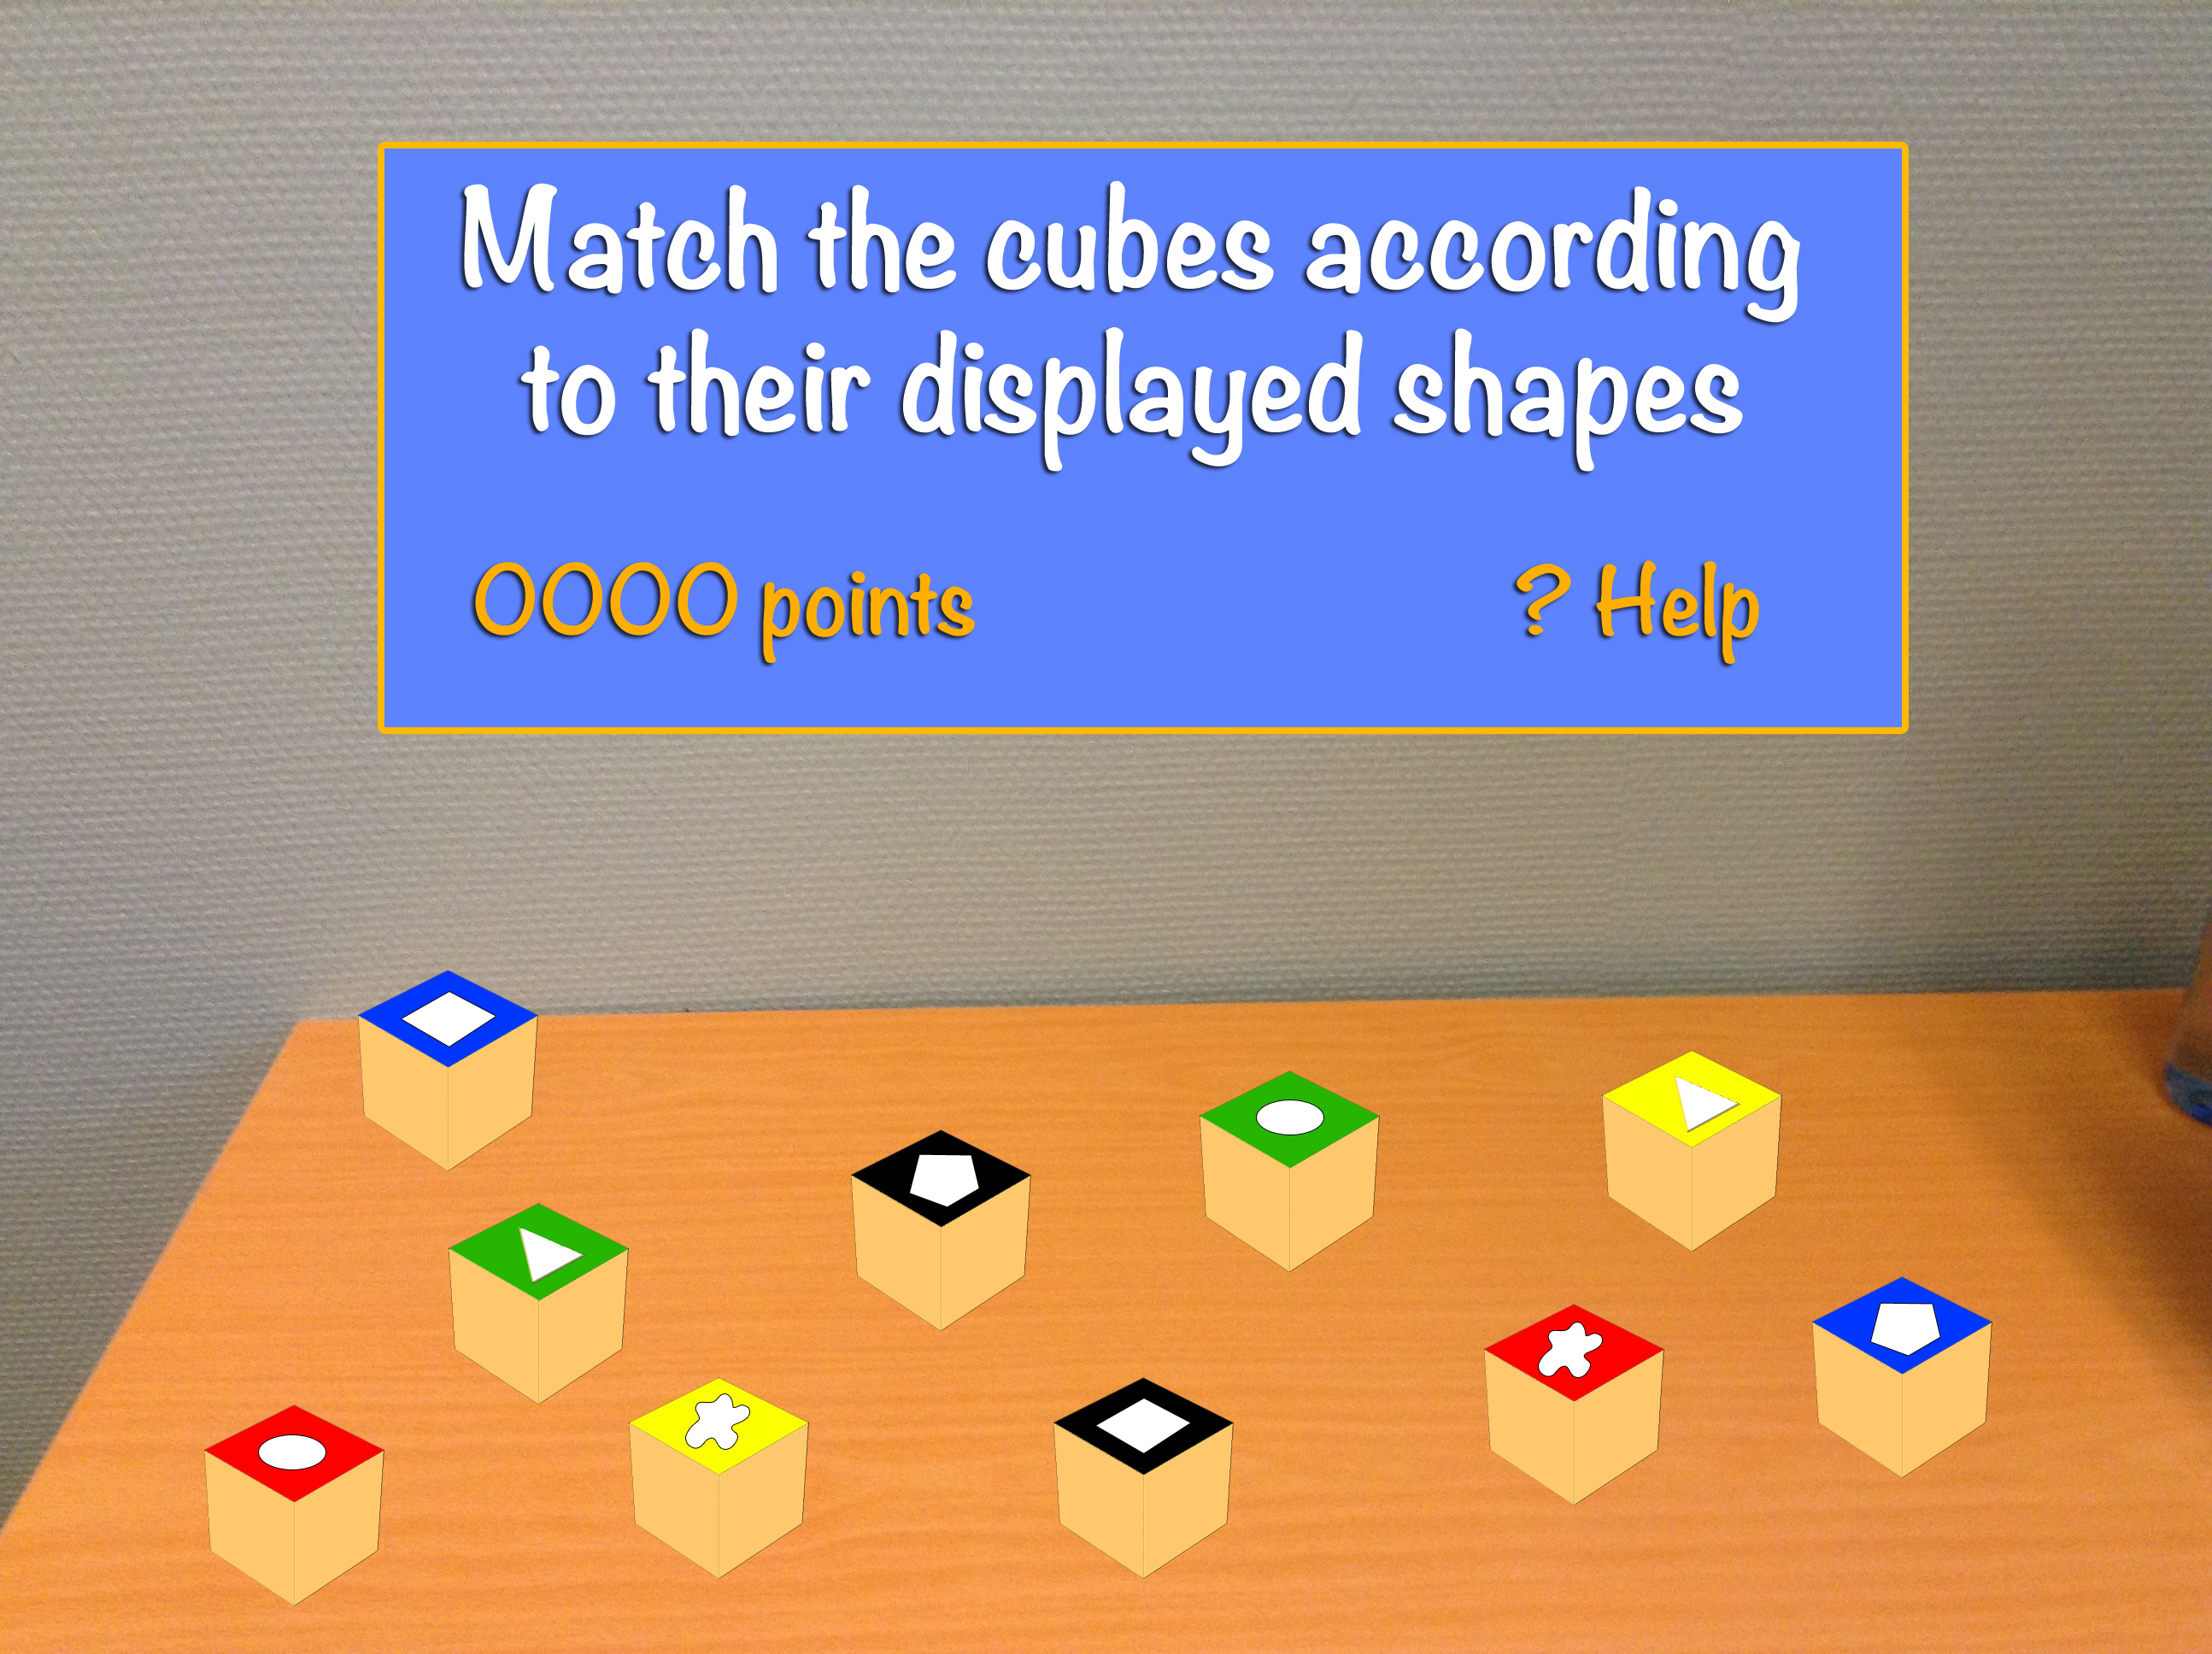
\includegraphics[width=0.9\textwidth]{images/Costas/game_mockup1(matching).jpg}
		\vspace{-10pt}
		\caption{Shape Match}
		\label{fig:Costas_shape_match}
	\end{minipage}%
	\begin{minipage}{.5\textwidth}
		\capstart
		\centering
		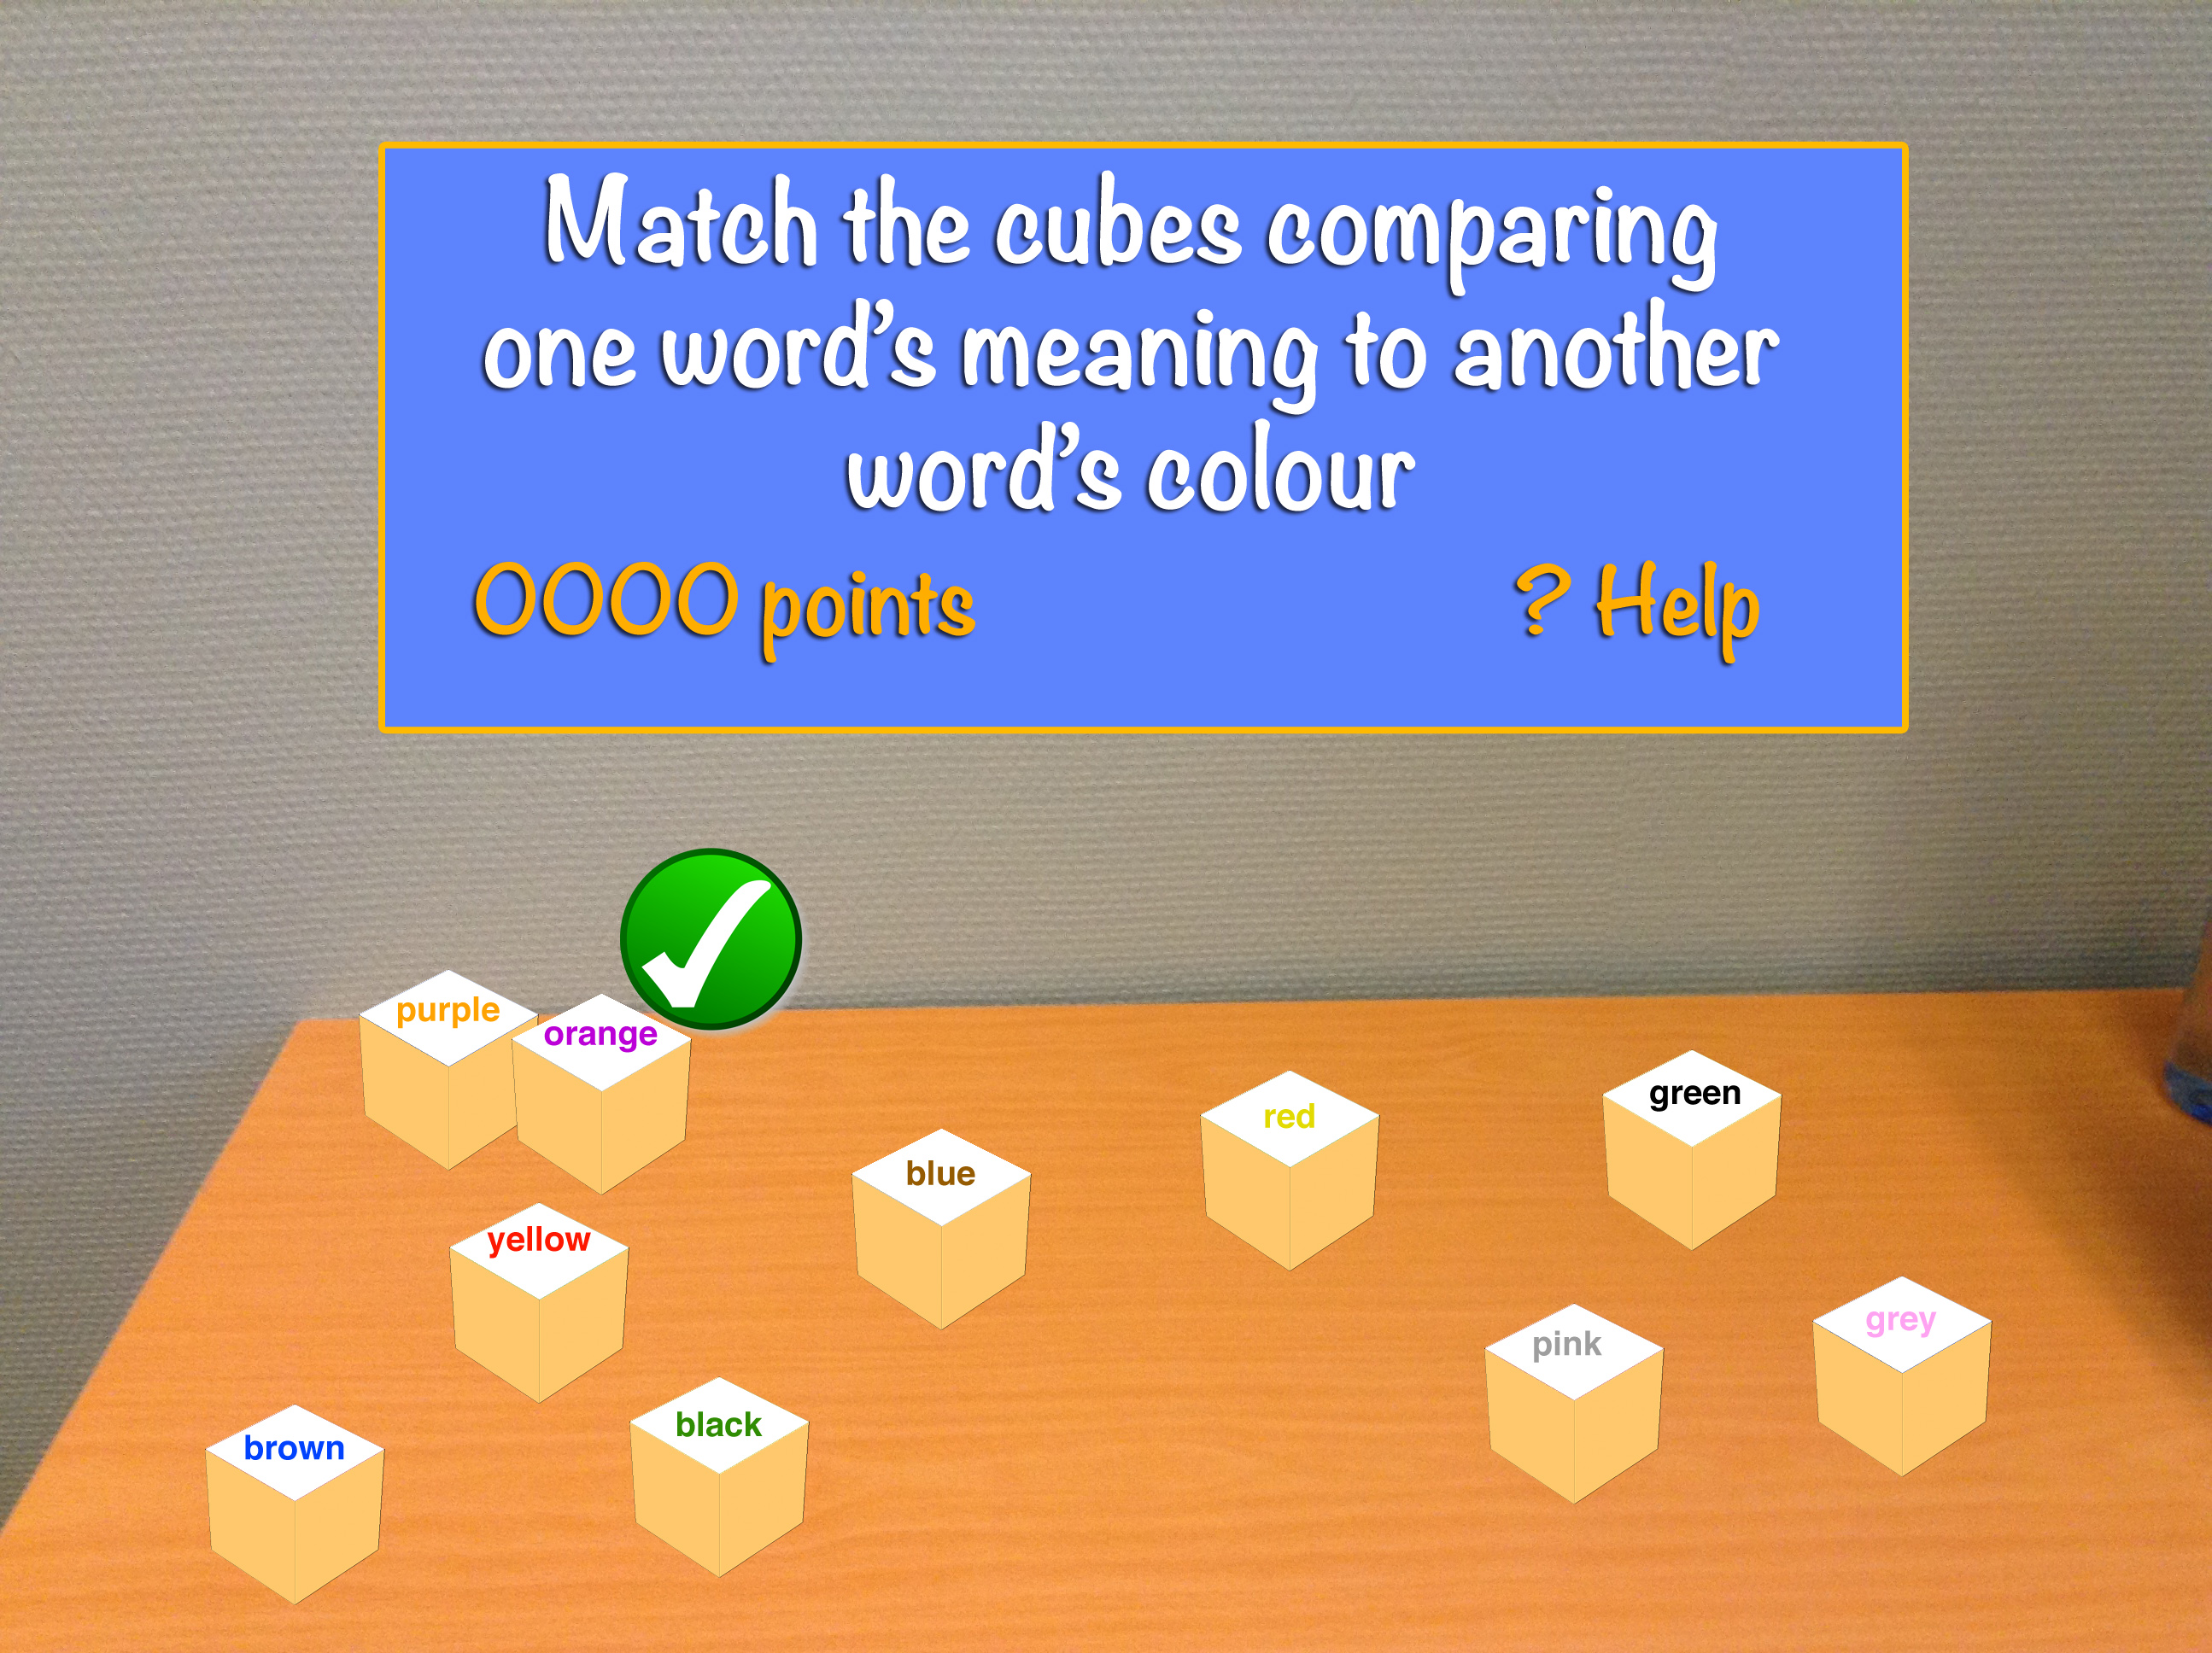
\includegraphics[width=0.9\textwidth]{images/Costas/game_mockup1(matching2).jpg}
		\vspace{-10pt}
		\caption{Colour Match}
		\label{fig:Costas_colour_match}
	\end{minipage}%
\end{figure}

\subsection{Shape Match}
	\label{game:shape_match} 

In this game the user combines pairs of cubes with matching patterns until all patterns have been found and put together.
The level is over either when all the pairs have been correctly placed together or time runs out.


\subsection{Colour Match}
	\label{game:colour_match}

This game also have users match up pairs of cubes, but instead of matching up figures and shapes the user have to pair up words and colours. For example one cube will have the text 'RED' written in a purple colour, and another box will have 'PURPLE' written in a red colour. The player have to pair up 10 cubes to a total of 5 pairs of such pairings.
The level is over either when all the pairs have been found or the time runs out.

\begin{figure}[h]
	\centering
	\begin{minipage}{.5\textwidth}
		\capstart
		\centering
		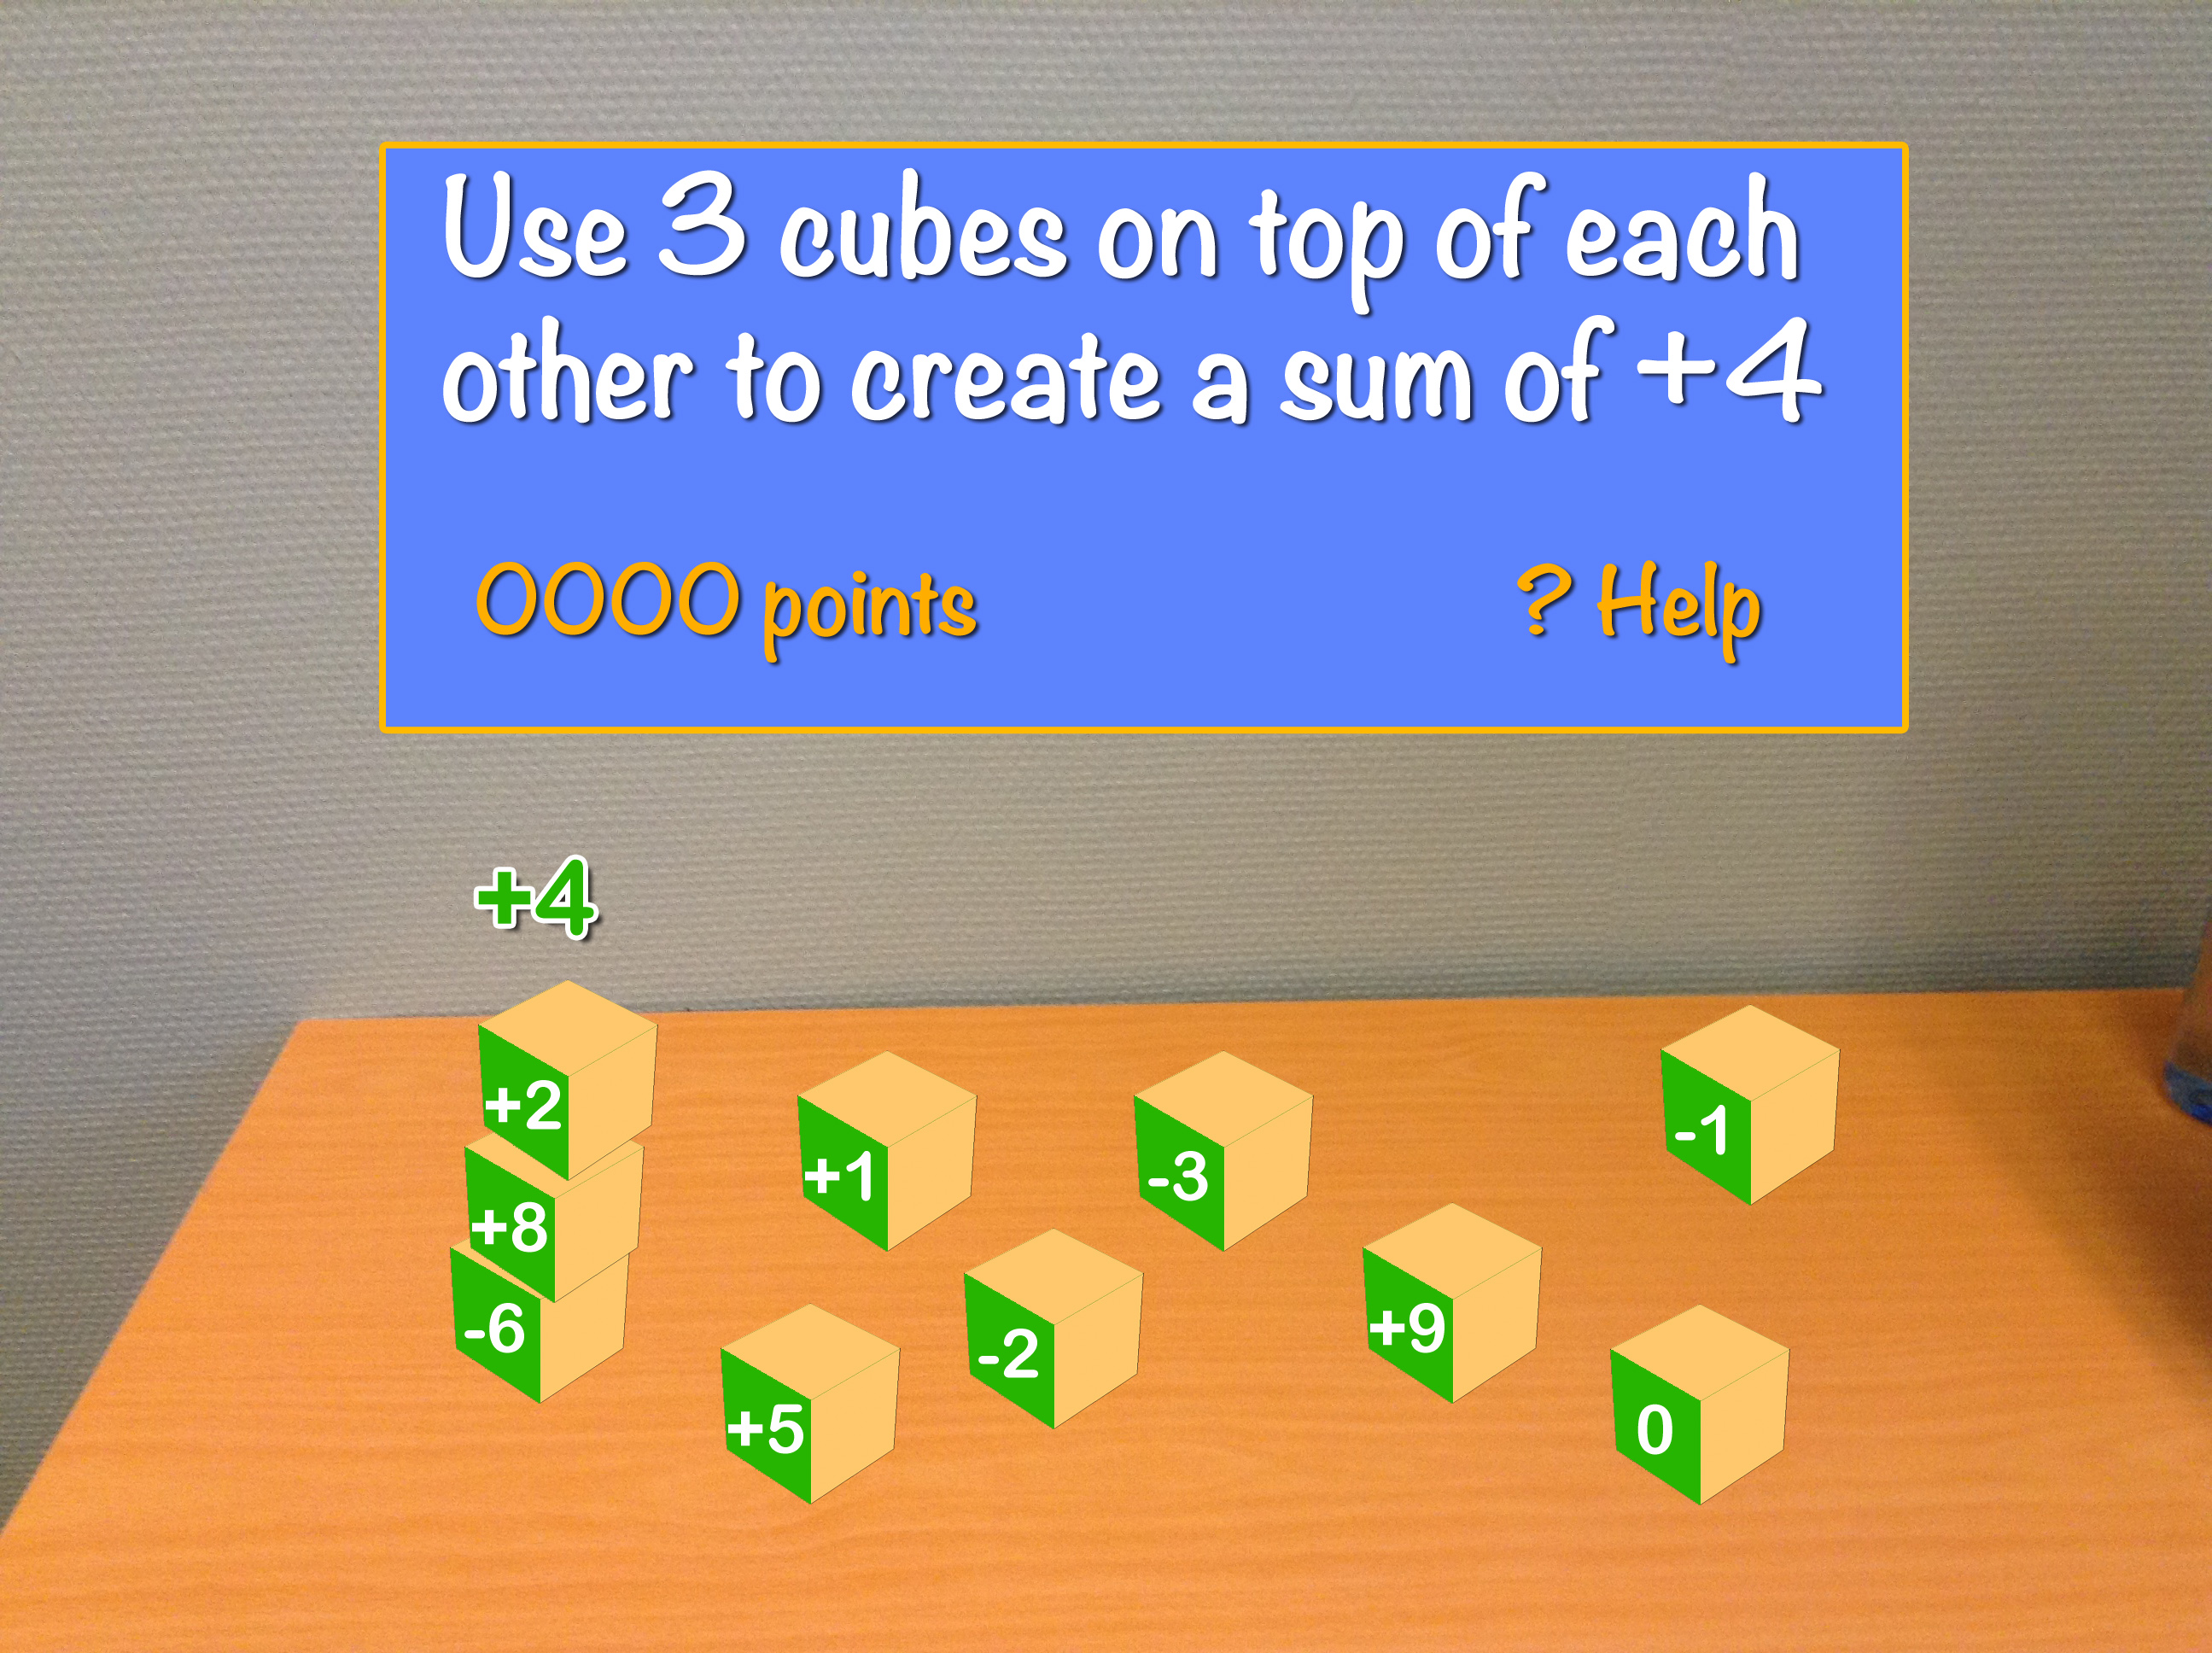
\includegraphics[width=0.9\textwidth]{images/Costas/game_mockup2(arithmetic).jpg}
		\vspace{-10pt}
		\caption{Total Sum}
		\label{fig:Costas_total_sum}
	\end{minipage}%
	\begin{minipage}{.5\textwidth}
		\capstart
		\centering
		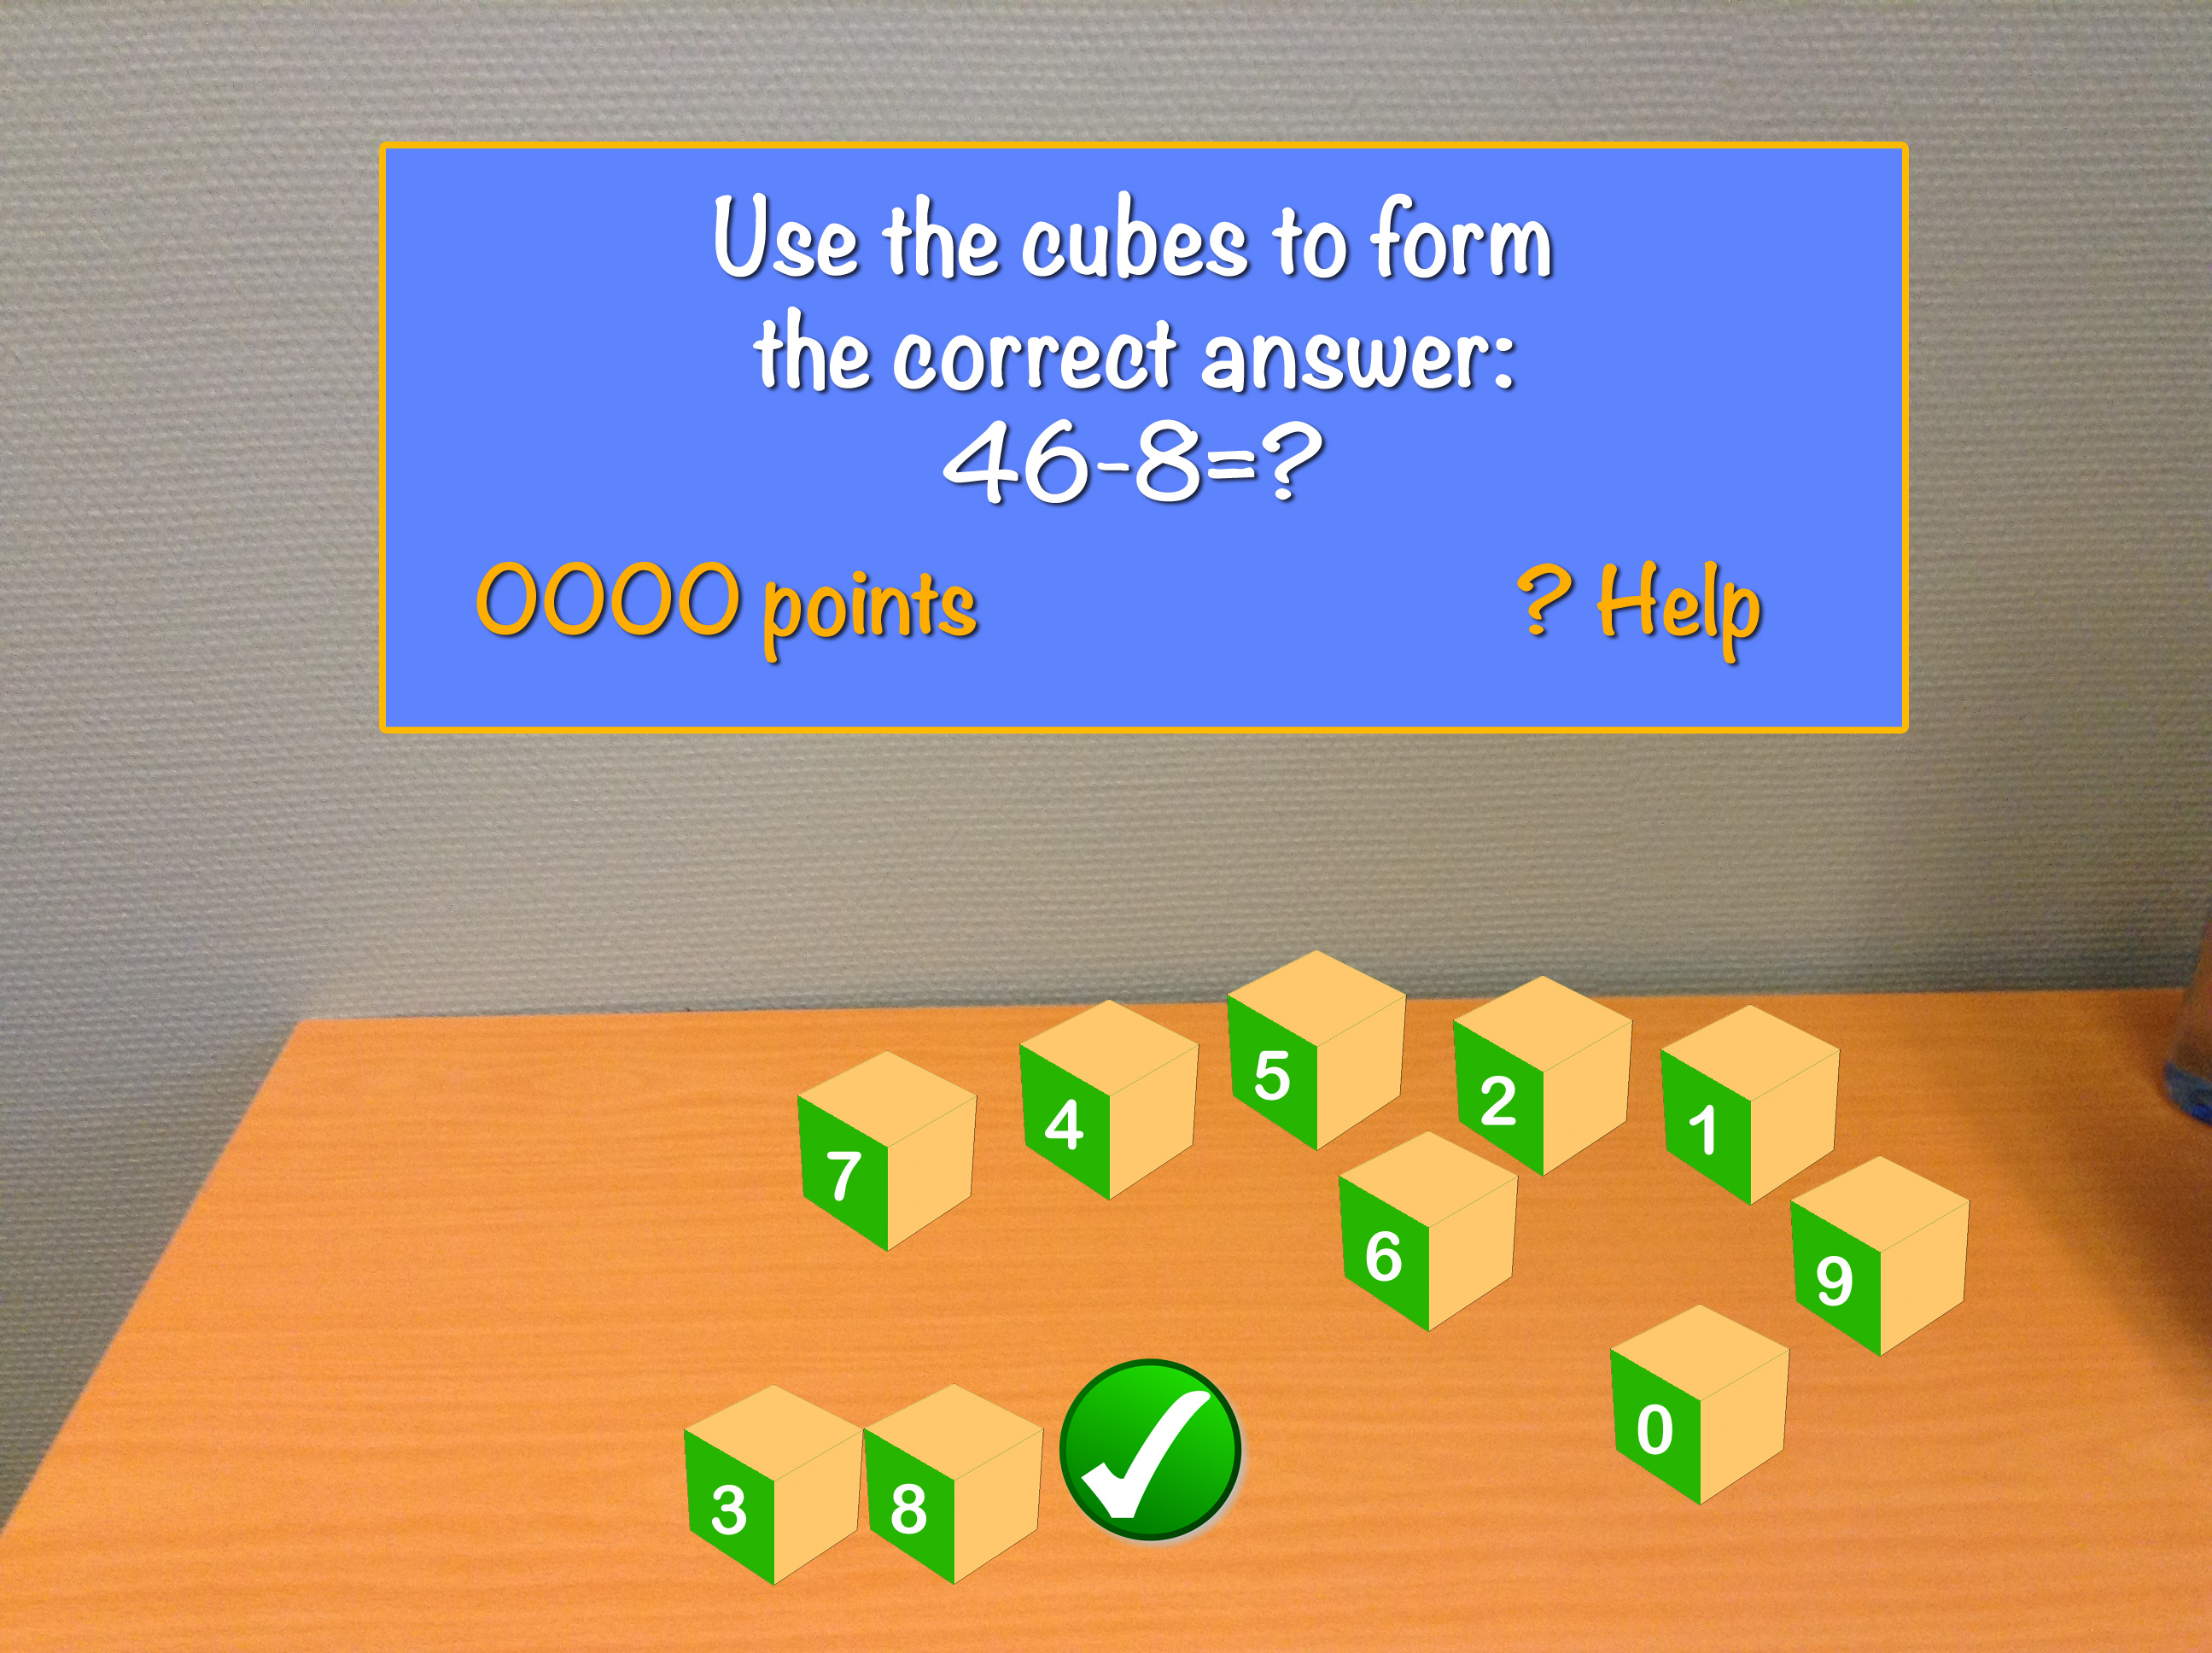
\includegraphics[width=0.9\textwidth]{images/Costas/game_mockup2(arithmetic2).jpg}
		\vspace{-10pt}
		\caption{Combining Numbers}
		\label{fig:Costas_combining_numbers}
	\end{minipage}%
\end{figure}


\subsection{Total Sum}
\label{game:total_sum}

At the beginning of each level in this mini-game the cubes all have different numbers on them, both positive and negative numbers. The goal of the game is to combine cubes in a tower so that they together create the number on the top of the screen.
The level is over either when the sum is found or the time runs out.



\subsection{Combining Numbers}
	\label{game:combining_numbers}

When the game starts the player is shown a arithmetic calculation problem that the player have to solve. Using two cubes the player combines them to show the answer. For example '36 + 6' will results in the answer 42 so the player have to place the cube with the number four and two next to each other to create 42 (but not 24).
The level is over either when the answer is found or the time runs out.

\begin{figure}[h]
	\centering
	\begin{minipage}{.5\textwidth}
		\capstart
		\centering
		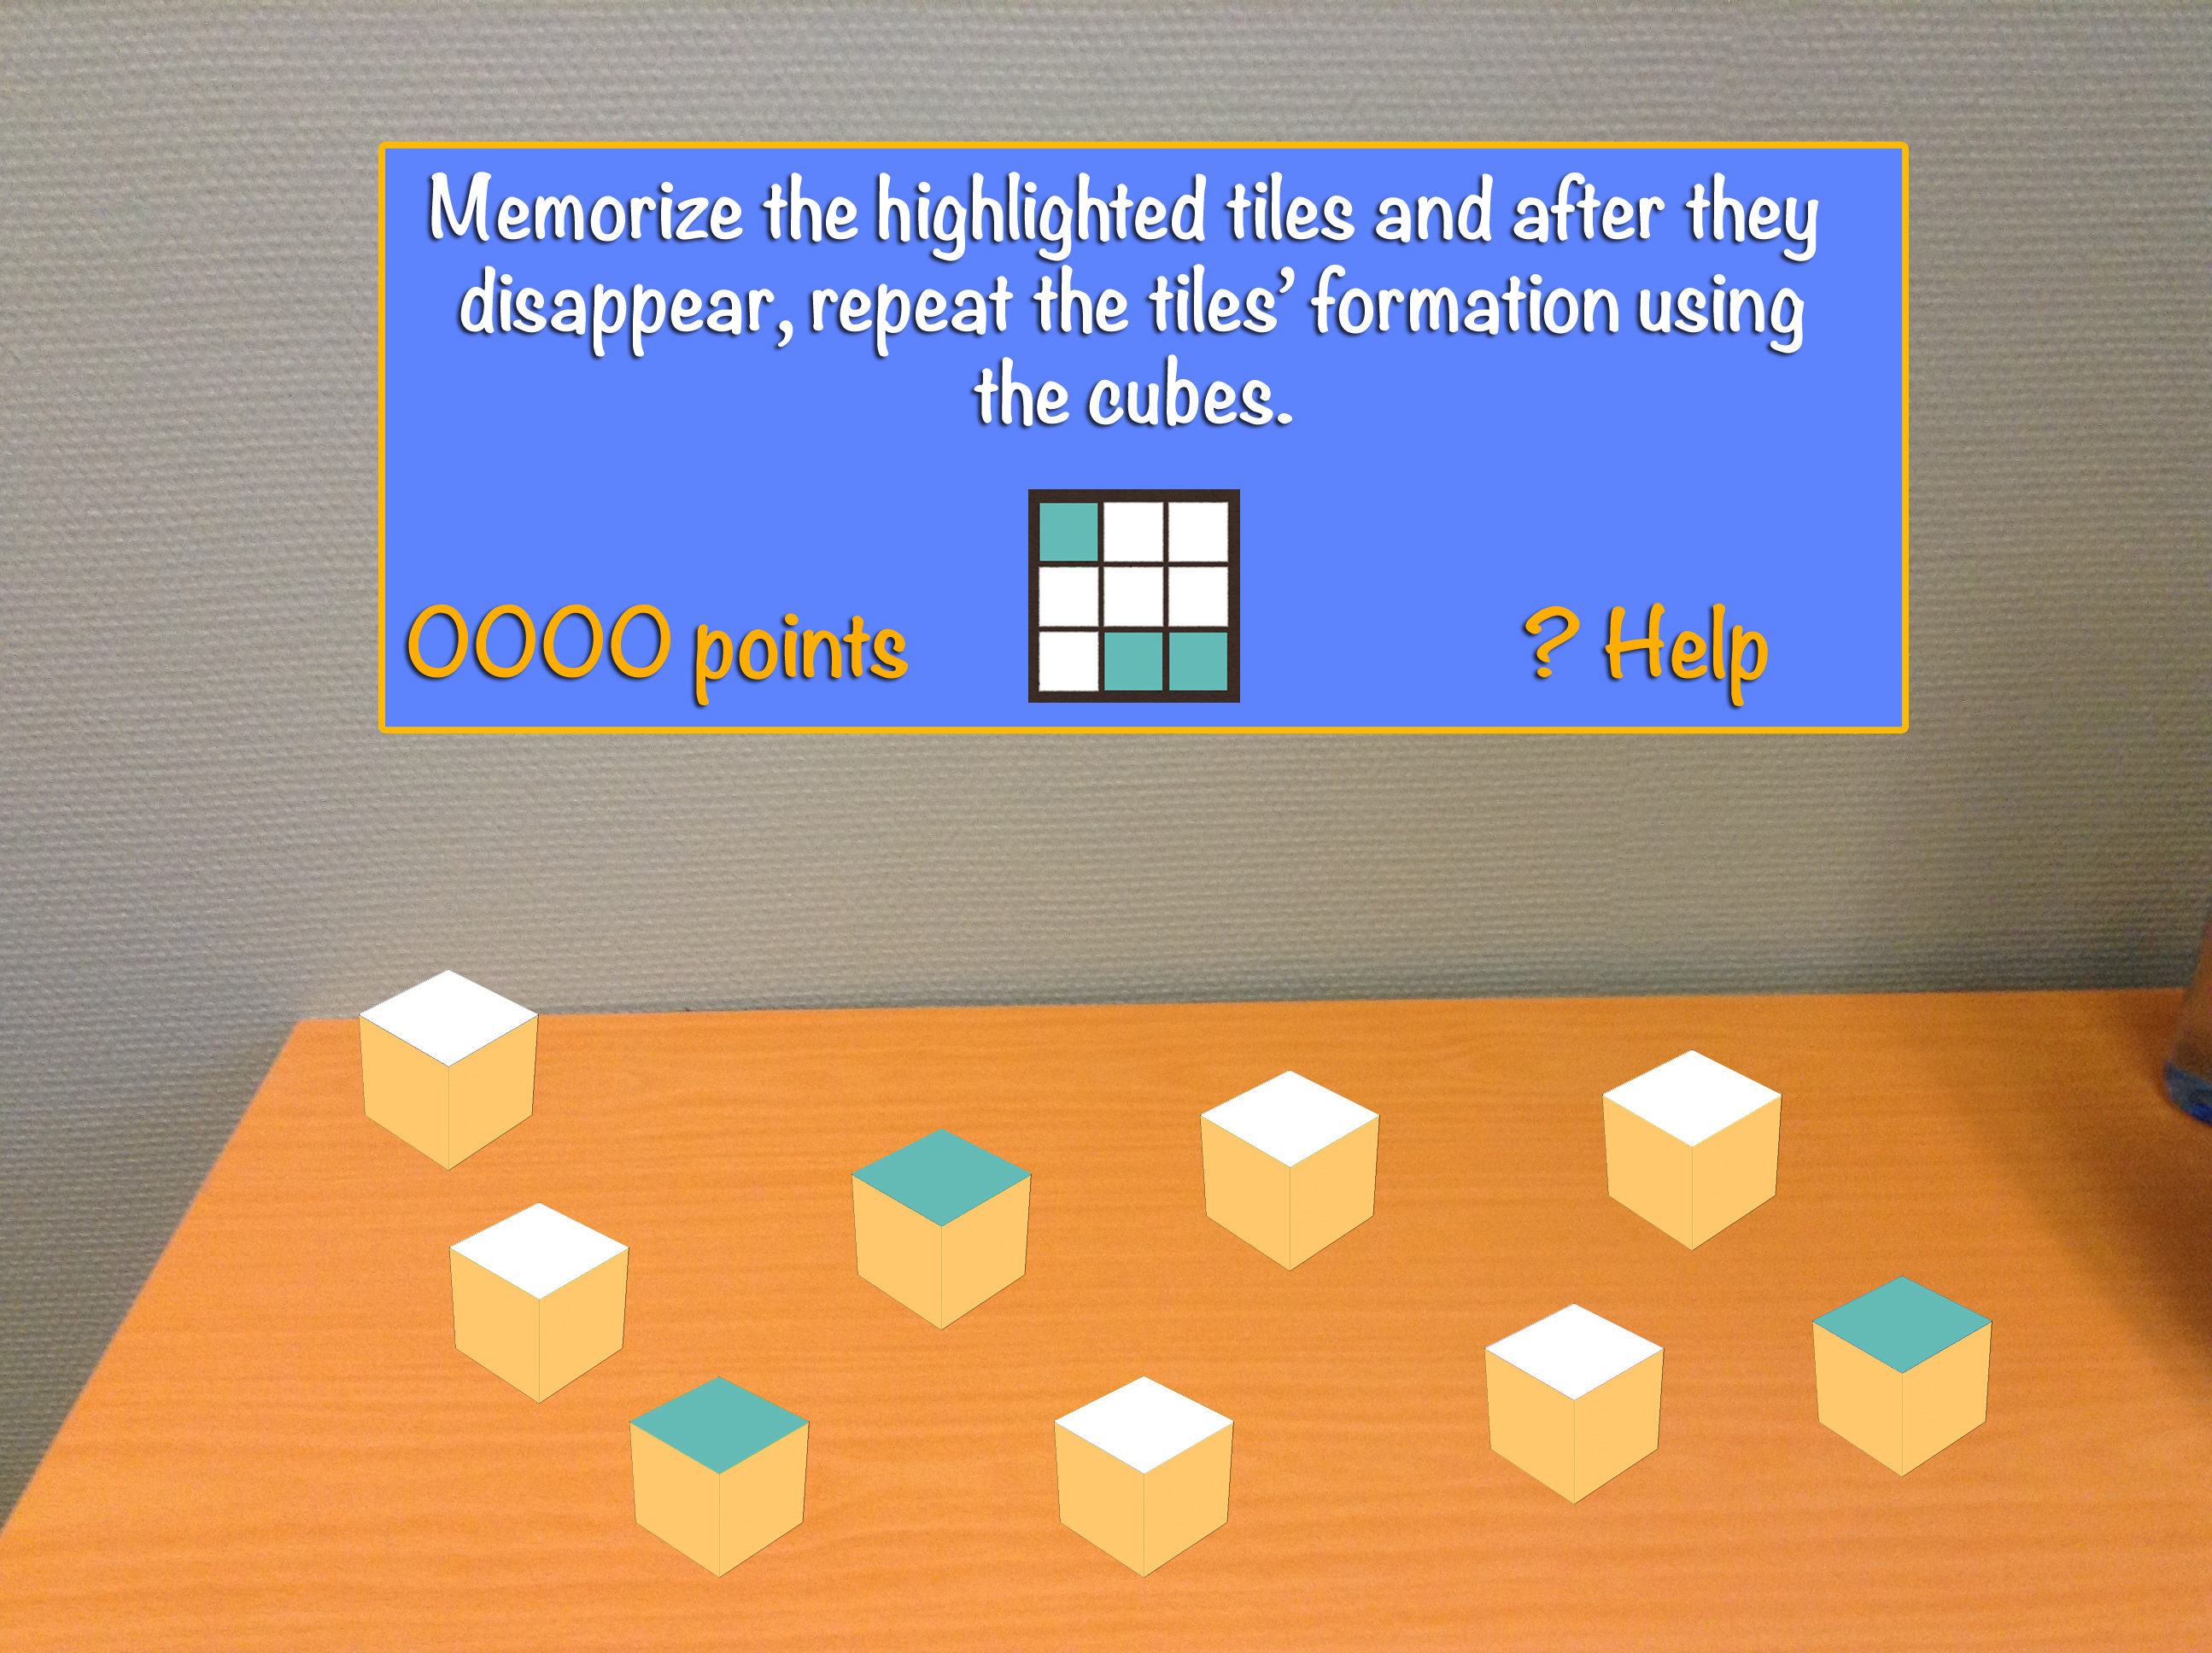
\includegraphics[width=0.9\textwidth]{images/Costas/game_mockup3(matrix).jpg}
		\vspace{-10pt}
		\caption{Pattern Memory}
		\label{fig:Costas_pattern_memory}
	\end{minipage}%
	\begin{minipage}{.5\textwidth}
		\capstart
		\centering
		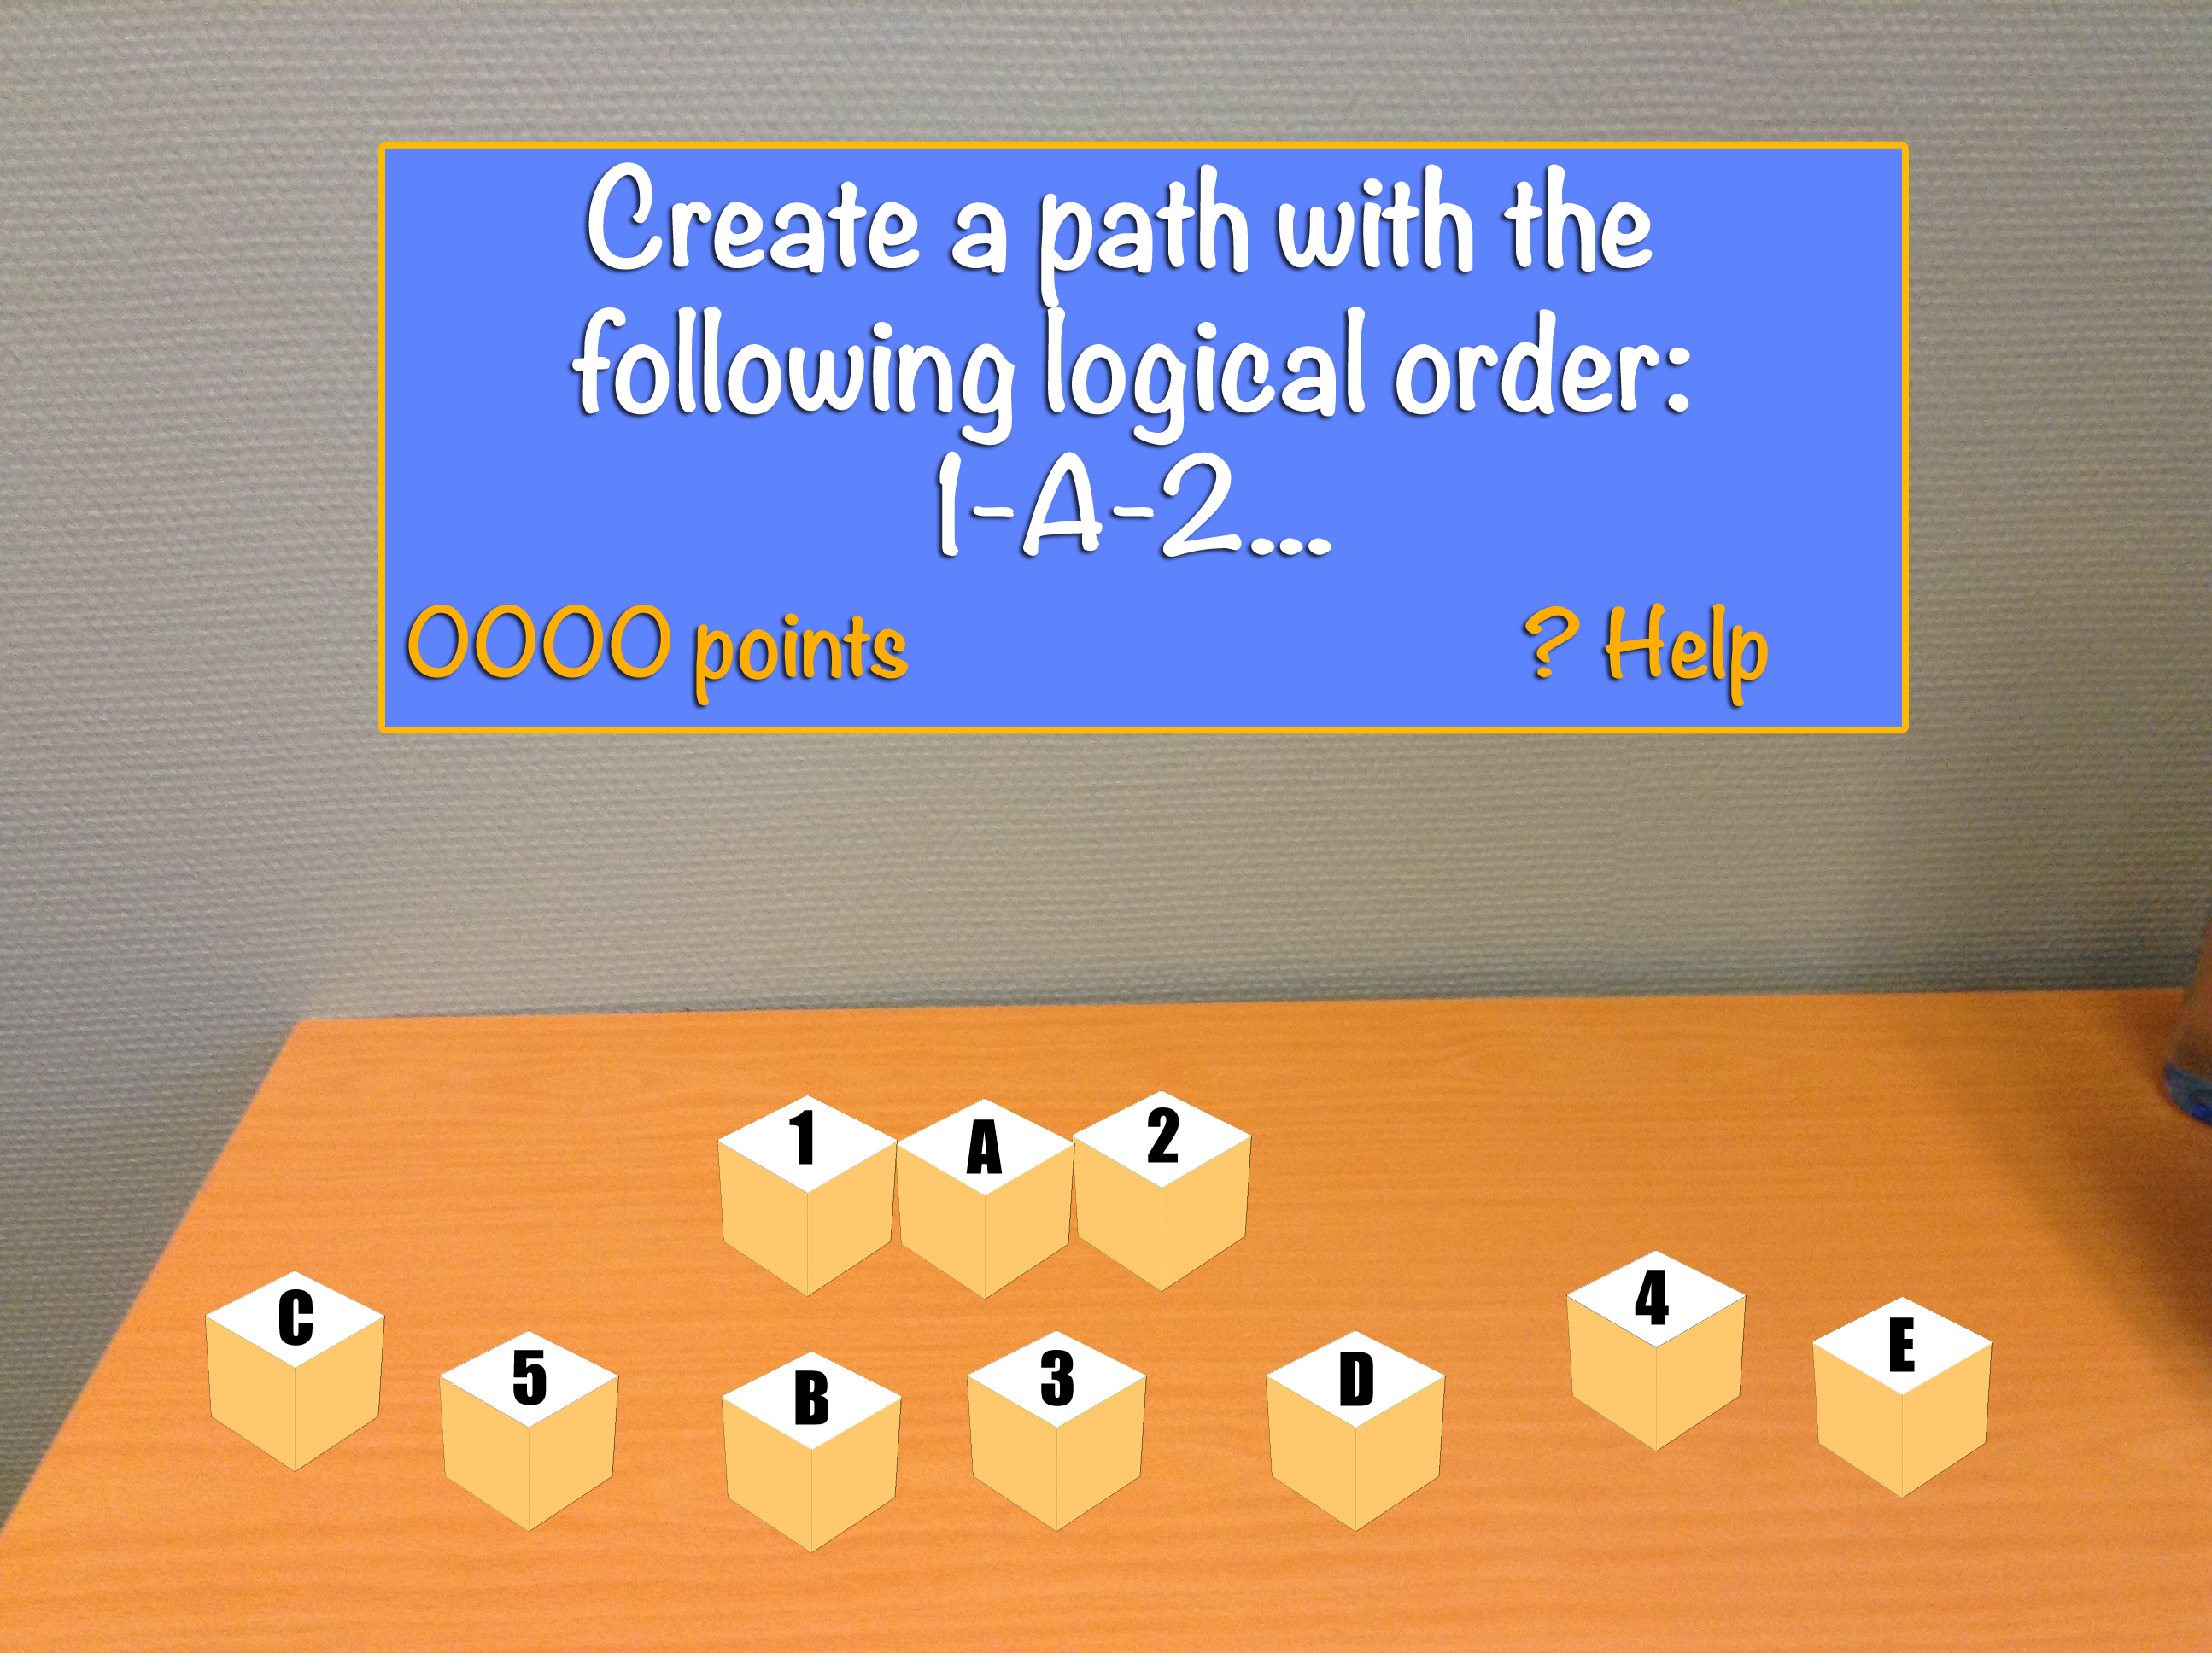
\includegraphics[width=0.9\textwidth]{images/Costas/game_mockup5(path).jpg}
		\vspace{-10pt}
		\caption{The Path}
		\label{fig:Costas_the_path}
	\end{minipage}%
\end{figure}


\subsection{Pattern Memory}
	\label{game:pattern_memory}

At the beginning of each level the player is shown a grid of nine cubes where the cubes can have two different colours, the goal of the game is to place the cubes in a grid making the same pattern as shown in the grid at the beginning of the level. The level is over either when the player have successfully recreated the grid pattern or the time runs out.


\subsection{The Path}
	\label{game:the_path}

Using the cubes the player have to make a logical path using all of the cubes. The five of the cubes have letters from A to E, and five have the numbers 1 to 5. The goal was then to make a line showing 1A2B3C4D5E. The game is over either when the path is completed or when the time runs out.


\begin{wrapfigure}{r}{0.47\textwidth}
	\capstart
	\centering
	\vspace{-20px}
	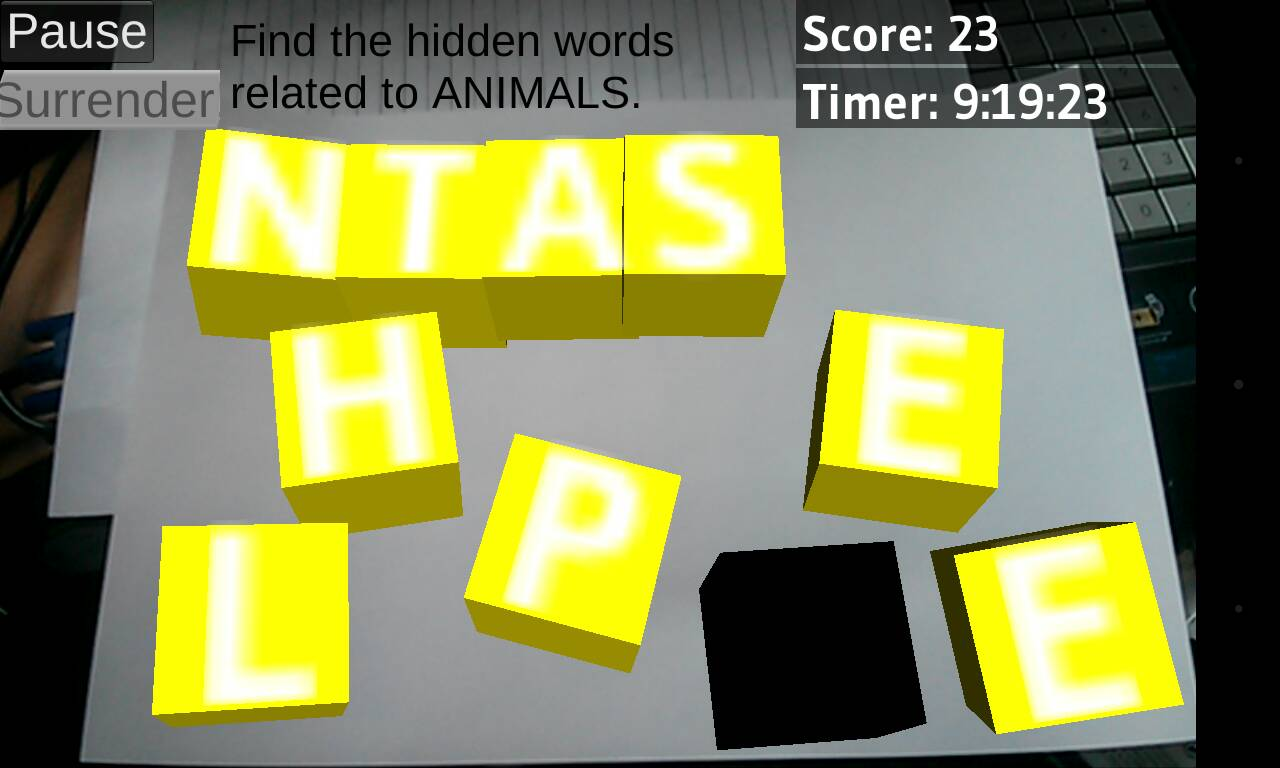
\includegraphics[width=0.45\textwidth]{images/Wo0ords_screenshot.jpg}
	\vspace{-10pt}
	\caption{Wo0ord Game}
	\label{fig:Costas_wo0ords}
	\vspace{-20pt}
\end{wrapfigure}


\subsection{Wo0ord Game}
	\label{game:wo0ord_game}
	
For this game the player is presented with a theme at the beginning of the stage, and using all the cubes which have letters on them combine them to make words related to the theme, the level is over when the player have either found 

	\chapter{Usability}
		\label{chap:usability}
		\subsection{Skipping levels}
During a game there might come up situations where you just want to quit. At
first we did not have this possibility, but during the testing phase we figured
out that this was something that had to be included. Particularly during the
Pattern Memory game (\ref{game:pattern_memory}) we think this is necessary. In
that game you will need to remember a pattern. If you fail to do so, you may
spend much time trying and failing to get the right pattern and frustration can
raise to an unfortunate level. 

\subsection{Total Sum Hint}
In the Total Sum game (\ref{game:total_sum}) it can be quite frustrating to add up the numbers in your head before hand, especially if the number of cubes you have to add up is more than three. When the player puts together two or more cubes in the specified way, (standard is vertical, but in the Unity inspector the rule can be changed to the horizontal version, "human readable" ) a text will appear on the top box or last box in the line showing how much the current sum is. The hint will only appear on one tower / word.

\subsection{AR Implementation}
AR implantation is explained in more depth in \ref{subsec:framemarker_model}.
When we were implementing Vuforia we focused on usability rather than aesthetics. The twitching, incorrect rotation and disappearing of the cubes when using the standard way give the player more nuanced feedback about the conditions for the tracking and understanding for how it works. Even though we were having tracking problems it was better to not make changes. There were other ways that could make the cubes easier to get into and keep in view, which would make some games easier to do if playing in bad conditions. but also in another way make the game harder because cubes would get stuck on screen or be in wrong positions confusing the player.



\todo{What have we thought through about usability? What can we make up here?}


\part{Development process}

	\chapter{Theory}
		\label{chap:theory}
		\subsection{Gyroscope and directional vectors}

\begin{wrapfigure}{r}{0.4\textwidth}
        \capstart
        \vspace{-20pt}
        \centering
        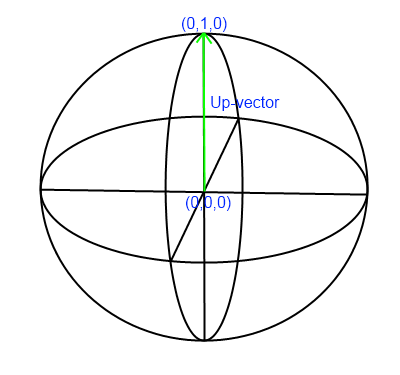
\includegraphics[width=0.38\textwidth]{images/GyroObjectModel.png}
        \vspace{-20pt}
        \caption[Model of the game-object used to get the direction up]{Not the one we used in the application, but it illustrates the principle better without the extra functions. This object is fixed in the real world when the user rotates the device, so that the up-vector points up in the real world.} 
        \label{fig:Gyro_model} 
        \vspace{-10pt}
\end{wrapfigure}

Since one of the games required the player to build towers with the cubes and since the project is about augmented reality, we thought it was a good idea to use the gyroscope rather than relying on the player to hold the phone the right way up. We also thought of using the gyroscope to separate four sides of interaction in the horizontal plane, but that is a compass and we couldn't expect the user to be facing north when playing the game. We could expect up to be up, but not west to be left, so for this we had to go with the unity-world-coordinates with the camera as center. The problem was to know how to use the gyroscope.\\

\begin{wrapfigure}{l}{0.4\textwidth}
        \capstart
        \vspace{-20pt}
        \centering
        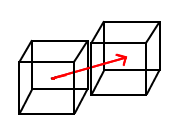
\includegraphics[width=0.38\textwidth]{images/CollisionDirectionObject.png}
        \vspace{-20pt}
        \caption[Model of the collision direction vector]{The vector shows the direction from the cube in focus to the colliding cube.} 
        \label{fig:Collision_Direction_model} 
        \vspace{-10pt}
\end{wrapfigure}

From a standard unity function we got the rotation of the real world from the gyroscope.The optimal thing to do would be to rotate the unity-world to be the same as this rotation. This however was not possible and the markers use global position so we couldn't make a virtual world object in unity to rotate. We could have added the rotation to the cubes transforms, but we only needed to know the direction of collisions. \\
We made an object that get its rotation directly from the gyroscope. To this object we added a child object that has a local position one unit above the parent. Subtracting the global position of the parent from the childs global position gives us a unit vector for the direction up in the real world. This could have been done more effeciently without the objects, but it was important to have visual indications of directions for development and testing.\\

\begin{wrapfigure}{r}{0.4\textwidth}
        \capstart
        \centering
        \vspace{-10pt}
        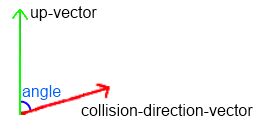
\includegraphics[width=0.38\textwidth]{images/CollisionDirectionAngleModel.png}
        \vspace{-10pt}
        \caption[Model for finding the angle between the vectors]{The angle between the up-vector in the gyroscope-object and the collision-direction-vector from the cubes.}
        \vspace{-10pt}
        \label{fig:Vector_Angle_model}
\end{wrapfigure}

Then on collision we can take the direction-vector between the colliding cubes. 
\[
(cubeB.position - cubeA.position)
\]

% This is the figure containing math. I put in some LaTeX math instead...
% \begin{wrapfigure}{l}{0.4\textwidth}
%         \capstart
%         \centering
%         \vspace{-20pt}
%         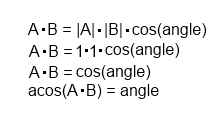
\includegraphics[width=0.38\textwidth]{images/AngleFormula.png}
%         \vspace{-20pt}
%         \caption[Description]{A = collision-direction-vector, B = Up-vector, |x| = length of x, cos = cosine, acos = arc-cosine.}
%         \vspace{-10pt}
%         \label{fig:Angle_Formula}
% \end{wrapfigure}

\subsubsection{Degree vertical}
By normalizing the vectors you can use the scalar product or dot product between the two vectors to find the vertical angle between the cubes. However Unity actually has a function for finding the angles between vectors, so most of our difficulty lay in testing that everything worked the way we thought and rotations were not inverted, incorrectly rotated or too unstable to use.


\subsubsection{Calculate the angle}
\newcommand{\norm}[1]{\lvert #1 \rvert}

For calculating the angle we need the following prerequisites.
\[
A = \text{Collision direction vector}
\]
\[
B = \text{Up vector}
\]
\[
\norm{x} = \text{length of x}
\]

\paragraph{}
With this in place we can get the answer with a little bit of math:

\[
A \cdot B = \norm{A} \cdot \norm{B} \cdot \cos(angle)
\]
\[
A \cdot B = 1 \cdot 1 \cdot \cos(angle)
\]
\[
A \cdot B = \cos(angle)
\]
\[
\arccos(A \cdot B) = angle
\]


\paragraph{}
 The angle varies between 0-180 degrees. We have specified that less than 60 degrees means one is below the other. More than 120 degrees means one is above the other. If the angle varies between 60 and 120 degrees, cogARC will see it as a horizontal collision.

	\chapter{Tools}
		\label{chap:tools}

		\section{Unity}
			\label{chap:unity}
			\todo{Why...?}
\todo{Generally how it works. Generally how it does not work. Generally how it make people cry.}

Unity is a game engine and development enviroment.
It features a intergrated work enviroment with good tools that promotes rapid workflows to create the games you wish to create without worrying about the underlying structure.
With its multiplatform deployment tools and intergrated asset store it has become very popular for games.
Supporting both 2D, 3D and animating makes so that you dont need other programs to create what you wish to create.

Getting into Unity for the first time is greatly aided by the many video tutorials that Unity has created, showing how to use the interface, basics of scripting and programming, how to add sound and much more.


		\section{Third party libraries}
			\label{chap:third_party_libraries}
			\section{PlayerPrefsX}
PlayerPrefsX (also known as ArrayPrefs 2)\cite{PlayerPrefsX} is a library created by the Unity community to enhance the built in Player Preference class of Unity.

PlayerPrefsX expands Unitys' way of storing player preferences or other data that the programmer want to persist between sessions.
Unity without PlayerPrefsX supports saving and getting float values, int values and strings. Altough this is all that is needed in most cases, it is sometimes practical to be able to store a bit more complex data.

PlayerPrefsX is able to store vectors, quaternions, arrays and more. 
We used this library to store the list of high scores for each game. 
By using PlayerPrefsX IntArray storing it was very easy to store a array of ten high scores for each game instead of having to either make a complex string to store it or fining another way of storing the scores.


		\section{Vuforia}
			\label{chap:vuforia}
			To achieve augmentation in our program without having to program it ourselves we used Vuforia.
Vuforia is a library that comes with packages for Android, iOS and as a Unity Extension.

Since we are using Unity it made using Vuforia a quite good choice.
Vuforia supports tracking of several different objects. It can track frame markers, image markers and simple geometrical objects.

The frame markers gets its name from their form. They are simple squares with a thick black outline with small squares of black or white around the inside of that square, the inner part of the frame marker can
contain anything the developer wish as long as the frame is clearly visible as Vuforia need to be able to detect the entire frame to activate augmentation.
Image markers can be more complex images and unlike the frame markers the image marker does not the entire image to be detected to activate augmentation.
If the image is clearly recognizable enough it needs only parts of it to be visible, we have seen demonstations where only half the image is visible and it is still able to track the image but it still need to see the entire image to begin the tracking.
Vuforia also supports cylinder targets and multi-targets which are image targets on cylinders or boxes such as a can of hairspray or a box of cereal where the logo can show augmentation such as product info.
And lastly it supports detecting and tracking of words, the words have to be between two to twenty-four characters long and not contain numbers.
It detects words based on a list of words and is currently supporting more than 100,000 English words \cite{VuforiaTextMarker}.

For our project we opted for the frame markers as we need to be able to track up to ten at a time without draining all the resources available as the program will be run primarily on a phone or tablet.
For tracking frame markers Vuforia does a very good job as long as the frame markers are clearly visible for the camera detecting it.

While Vuforia does a good job at tracking and finding frame markers it is still lacking in other areas.
One of the biggest difficulties we had with Vuforia was the lack of documentation, insight into how it works and ability to manipulate the behavior of Vuforia.
This is closely related to some of our problems during development as to what happens when Vuforia loses the tracking of a frame marker  that is clearly visible
 to the camera and should be able to track it.
We are not completely certain but we have experienced that lighting condition is what plays the most important role in this.
What is normaly done for making Vuforia augment an object in Unity is that you add the frame marker into the scene that you want Vuforia to be able to track and as a child of that frame marker you 
put the object(s) you want visible when Vuforia finds the marker.



		\section{MonoDevelop}
			\label{chap:monodevelop}
			MonoDevelop is the integrated development environment (IDE) that comes with Unity. It supports writing in C\#, Unity JavaScript and Boo.
MonoDevelop is developed by Xamarin \cite{xamarinRef} as an open source integrated development environment for Windows, Linux and OS X.
Its primary focus is on C\# and other .NET languages.


MonoDevelop offers debugging features such as breakpoint, stepping trough code one line at a time, tracking of variables, call stack of functions and more.
It also have features to help with programming such as code completion and solution overview. Alongside all this it also supports add-in's for adding support for other languages.


\begin{wrapfigure}{l}{0.3\textwidth}
	\capstart
	\centering
	\vspace{-10pt}
	
\includegraphics[width=0.28\textwidth]{images/MonoDevelopLogo.png}
	\vspace{-20pt}
	\caption[MonoDevelop IDE Logo]{{M}ono{D}evelop {IDE}}
	\label{fig:monodevelop}
	\vspace{-10px}
\end{wrapfigure}

For us MonoDevelop gave mixed results. 
I have no doubt that it is a good IDE for working with C\# or a .NET language, but the UnityScript integration is poorly done.
The auto complete functions was flimsy at the best of times, most of the time it never activated and when it did it did not give the correct results. 
There has also been times when trying to get a public variable have resulted in a error because the variable has yet to be defined while it is available two lines above with no change in the scope.
We believe these problems are more due to Unitys implementation of JavaScript and not a error on MonoDevelops part, so if one are to use MonoDevelop we would recomend to shy away from Unitys JavaScript and use C\# instead.
Ending with on a positive note it had the best "Watch" feature we have come accros, it made tracking of several variables at a time really simple even if that variable was part of another script or class.	

\todo{Does this need more?}

		\section{GIT}
			\label{chap:git}
			We have been using GIT for version control in this project. This is a version
control system we had some prior experience with, so we wanted to try it for 
this project as well. 

GIT works best with plain text files. With Unity there is quite many binary
files as well. At first we were not entirely sure how much of the files that
were binary and if GIT could work for us. After some googling we found that 
this was possible. On Unity's webpage they instruct on how to use the version
control system called Subversion \cite{SubversionControl}. Together with some
help from stackoverflow.com\cite{gitVersionControl} we figured out how to set 
up the project with GIT.

Unity produces .meta-files for each file in the project. We do not know 
entirely how these works, so we met some problems that we suspected had its
origin in these files. Because of this we have tried both to have them in
the GIT repository and not. The solution to that specific problem was not
clear when we got it working, so we do not know whether the metafiles were
problematic or not. The post at stackoverflow explained that the .meta-files 
could be set to hidden. This implies that the files should not be part
of the GIT repository. Anyway, now thay are because it seemed to help with the
problem we had, and it has not given any other problems later.


\begin{wrapfigure}{l}{0.3\textwidth}
	\capstart
	\centering
	\vspace{-10pt}
	
\includegraphics[width=0.28\textwidth]{images/git}
	\vspace{-5pt}
	\caption[GIT logo]{GIT}
	\label{fig:git}
	\vspace{-10pt}
\end{wrapfigure}

Many of the pure binary files has not been necessary to upload. Those that
has, like images, has often been of a type that didn't need to be updated
often. This means that most of the content in the repository could be plain
text and therefore we have been able to use GIT without further hassle.

\begin{wrapfigure}{r}{0.3\textwidth}
	\capstart
	\centering
	\vspace{-10pt}
	
\includegraphics[width=0.28\textwidth]{images/github}
	\vspace{-5pt}
	\caption[{G}it{H}ub logo]{{G}it{H}ub}
	\label{fig:github}
	\vspace{-10pt}
\end{wrapfigure}

We have used GitHub \cite{GitHub} as our online repository server. By using
this service we could easily share the work we have done. That we could use
an external server like this has been important for us when choosing version
control tool. Especially in one occation this proved to be very smart. One of
us encountered a bug in Unity that were quite severe. The Unity3D program
crashed, and by some unknown reason, it deleted a lot of files. The files that
were removed were all of the project files + some other files in the parent
directory. Many totally unrelated files were deleted and 4 days work that was
not committed to the server were lost. But fortunately enough, he could
download the lastest version from GitHub and use the last days lessons to write
the lost changes a whole lot faster.

When we have been using GIT we have used the commandline tool and also the GUI
program for GIT called Sourcetree \cite{SourceTree}.

The workflow we have been using has been very simplistic. We are aware that
there are good workflows that we could have used, but we have choosen to only
have a master branch that everyone pushes to. During the project we were told
about a way that worked for another group were they used pull requests and in
this way added an extra layer of security of code integrity. We tried this out
for a short time, but since none of us had experience with this way of working,
we discared it after a relatively short time. We were working quite close with
many small and rapid changes that we shared with everyone. If another group
member should accept this every time, we think that a lot of unnecessary time
could have been wasted on this. The model is not bad, but we have come to the
conclusion that it didn't fit our way of working very well. If we had started 
to do it from the beginning, we could maybe have done it, but the effort may
still have not been worth it. Anyhow, we are glad to learn about other ways of
working that can be useful later.

		\section{LaTeX (\LaTeX{})}
			\label{chap:latex}
			We have chosen \LaTeX{} as the tool for writing our report. In the preplan we
made the document with Google Documents \cite{GoogleDrive}. This worked ok, since
we all could work with the document at the same time. The functionality in that
editor is quite ok, but somewhat limited and hard for big projects. One is
also dependant on a stable Internet connection. 

\LaTeX{} on the contrary, is a tool used to create books, articles and reports.
It can handle many pages and is therefore a good tool for our purpose. \LaTeX{}
documents are compiled from clear text files which makes it easy to use GIT and
work with it as any other programming project. The report document have been hosted
on GitHub so that we could work with it offline, but share our changes online
when they are ready.

Since none of the group members had any notable experience with \LaTeX{} 
before, we used some time on deciding whether we should use it or not. It takes
some time to learn and get used to \LaTeX{}, but after we had been using it for
a while, we learned to like it more and more. We will encourage readers to give
it a try as well.


	\chapter{Schedule}
		\label{chap:schedule}
		We planned the development project and ended up with the gantt diagram shown in Figure \ref{fig:preplan_gantt}:

\begin{figure}[h]
	\capstart
	\centering
	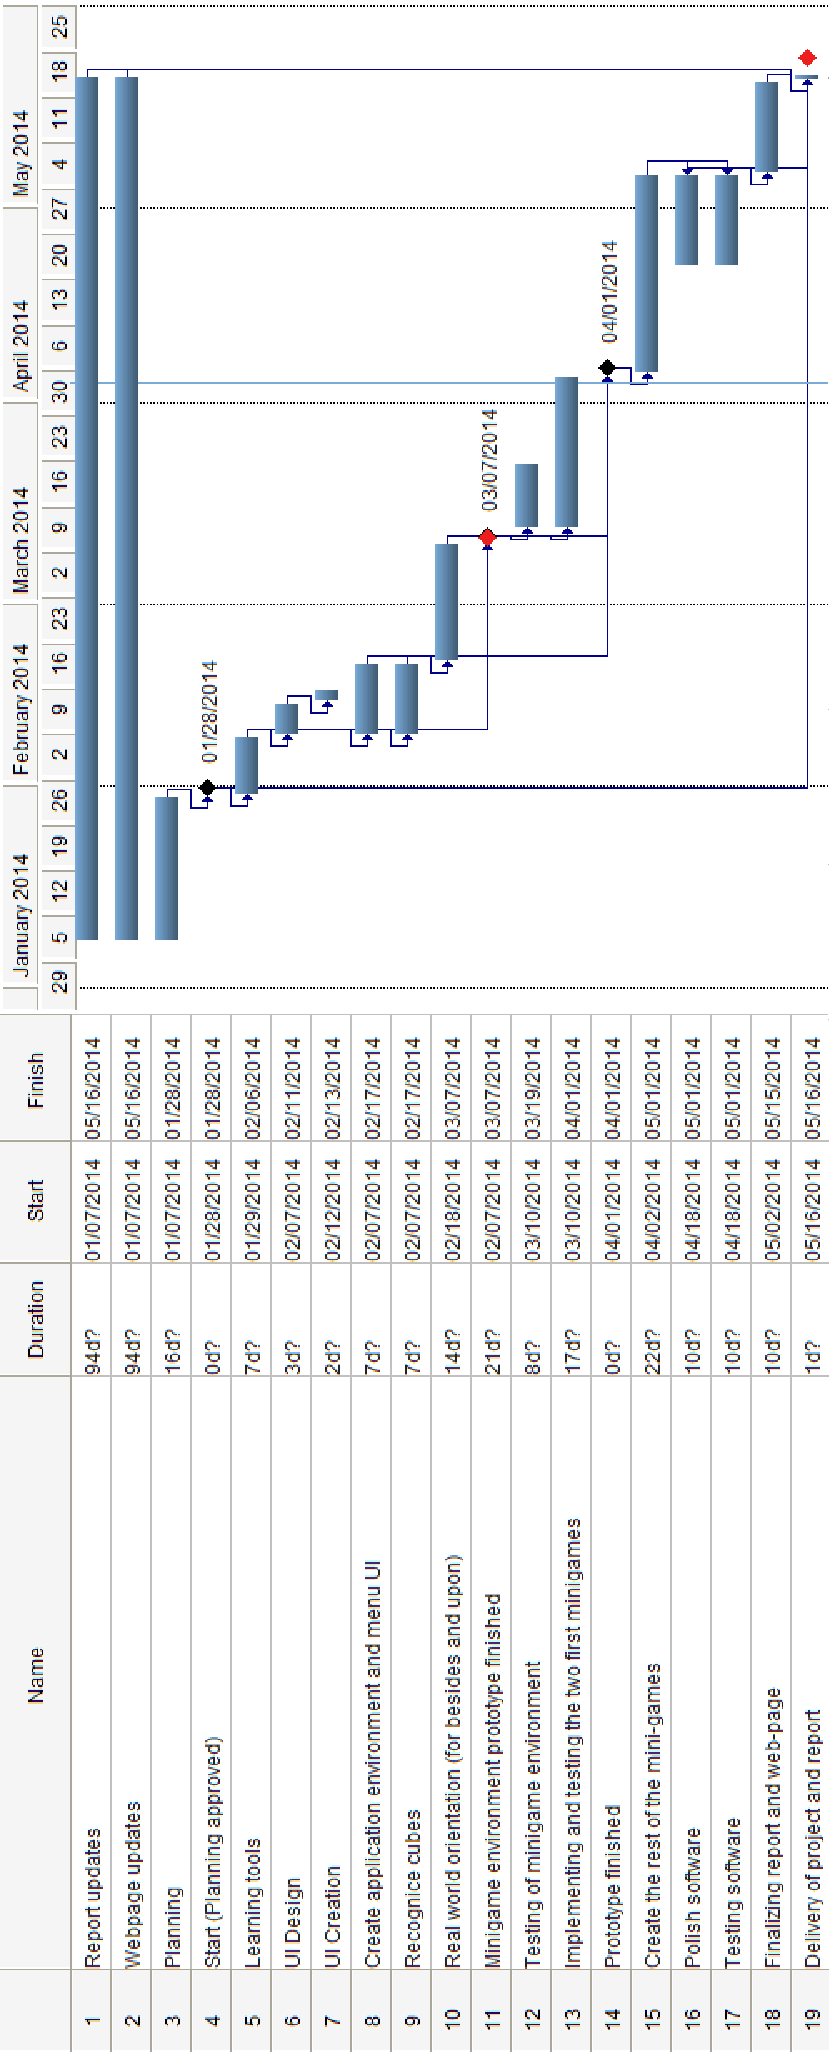
\includegraphics[height=\textwidth, angle=270]{preplan_gantt_diagram}
	\caption[Preplan Gantt diagram]{Our initial gantt diagram for the project.}	\label{fig:preplan_gantt}
\end{figure}


Afterwards we see that the process has been like this:

\todo{Insert gantt diagram of our dev-process here.}

\section{Planning vs reality}%Or how we worked compared to the plan
Our development cycle deviated a lot from the original plan due to a multitude of factors.
For instance we could have allocated less time to the "Create application enciromnet and menu UI" and "Recognice cubes" which each were allocated 7 days in the plan, but had we known more about Unity or the Vuforia plug-in in Unity then we would have known that Unity have methods and functions for creating in-game UI and to make the Vuforia plug-in working were just adding a \gls{prefab} for the camera.
We spent the time allocated to those time slots to creating the framework instead and this additional time shifted a lot of the sub-sequential work a week ahead of time.
Task number 10 (Real world orientation (for besides and upon)) was moved to the beginning of the project by developer Jakob and was done as part of him learning Unity.

The most drastic change in the time schedule is in item 11-15.
After learning some of the inner workings of Unity and how to properly set up a game in Unity it became rapidly apparent that we had taken a somewhat naive approach on it. This was due to our lack of knowledge of how much a game engine can do for us.
Using Unity we had a almost complete mini-game enviroment from the beginning. As such we only had to program what interaction we wanted to happen when cubes collided.
Our time and efforts were then spent on making the interaction between cubes and the player to what we wanted instead of having to focus on making the basics of a game world working.


	\chapter{Process}
		\label{chap:process}
		\section{Development process}


	\chapter{UnityScript}
		\label{chap:UnityScript}
		In Unity a user can use several different languages to script their games. Boo, C\#, JavaScript and Shader (used for writing shaders).
While Boo and C\#  use the standard implementation and is easily referenced the JavaScript used in Unity is not.\cite{WikiScriptVSScript}

Unitys JavaScript is quite different in many ways from the more standardly used JavaScript that is based on ECMAScript\cite{ECMAscipt} which is a standardized scripting
language standardized by Ecma International.

Some of the major and notable differences between Unitys JavaScript (henceforth named UnityScript) and ECMASCripts JavaScript (henceforth refered to as JavaScript):

\begin{itemize}
	\item Classes.
	\item Different privacy.
	\item var as a keyword is required.
	\item Not JavaScript library compatible.
\end{itemize}

\section {Classes}
JavaScript have no concept of classes as it is a prototypical language, meaning it will have the properties that is assigned to it, but is not bound to them.
Properties can be added or deleted at will in runtime, this is true for both members of the object and functions. UnityScript is much more object oriented with strongly typed and defined classes that cannot be changed in runtime (the exception to this rule is reflection).
This makes it difficult to work with UnityScript if you have little experience using it, or have yet to find out that the difference between JavaScriptand UnityScript.
UnityScript have also removed the prototypical properties of JavaScript by implementing it as a class based language. Meaning objects can not get additional functionality or be completely redifined at runtime. In UnityScript each .js file is implemented as a class by default. So when a developer creates a new .js file the Unity compiler and serialization system will add a class definition around the data within the file by default, so to call a funciton within a .js file you write "filename".function.

\section {Different privacy}
UnityScript, being structured like other object oriented languages have the usual levels of privacy of members within a class being markedas either Private, Protected or Public. JavaScript have per function privacy. Meaning a variable declared in a function is available in the entire function but not outside of the function.

\section {var as a keyword is required}
If you do not use the keyword var in JavaScript the variable becomes a global variable as the var keyword is used to denote scoping. In UnityScript the var keyword is required when creating a variable to make sure the scoping is always the intended scope.

\section {Not JavaScript library compatible}
UnityScript being so different from JavaScript makes other pre-made JavaScript library non-compatible with UnityScript, which also makes it really difficult to find reference help. One half of the built in library in Unitys Monodevelop is Unitys own library and the other half is made using what seems to be .NET framework from MicroSoft


	\chapter{Unity Serialization}
		\label{chap:UnitySerialization}
		Unity operates with two memory spaces. The native one belonging in to the C++ side of the code and the more managed DLL side that comes from scripts.
The managed side memory is where all the data from scripts that we as users are put.
To use the data Unity does something called assembly reload. What happens it that it pulls all the data out of the managed side, creates an
internal representation of the data on the C++ side, destroys all the memory from the managed side, reloads the assemblies and then
re-serialize the data from C++ into the managed side.
The serialization happens when the Editor or the system reloads an assembly, when the user enter and /or 
exits play mode and when the scene is loaded/ saved.
A serialization can therefore happen rather frequently or rarely, depending on the work-flow of the user
 and what the user is currently doing.
This is all well and good, until you get into one of the few corner cases where your data does not serialize into C++ and gets destroyed.

Unity is only able to serialize basic data types and those already defined within the MonoDevelop system that is part of Unity.
What this means is that if Unity does not know explicitly that the data are to be serialized or if it is unable
to serialize it, it will simply be destroyed. Most classes will not be serialized unless they have data that Unity 
can recognize is being used.
There are a few ways to make sure Unity knows that the data shall be preserved not destroyed:
\texttt{enumerate}
\begin{enumerate}
	\item Make the data field public
	\item Mark the field as serialize-able (@SerializeField in JavaScript and [SerlializeField] in C#)
	\item Mark the class as serialize-able (@Serialize in JavaScript and [Serialize] in C#)
	\item Make a class that derives its base type from ScriptableObject
\end {enumerate}

By having the data marked in either of those ways or a combination of them will ensure that Unity will try to
serialize it.
But there are a few things that Unity can not easily serialize, and most notably it can not serialize an array of normal objects.
It can serialize an array of objects that is derived from ScriptableObject. What the serialize will do is serialize each object in the
array individually and put a pointer into the array. To make this work the ScriptableObject derived class has to be in its own
C# file.
Unfortunately for us we are using the Unity engines JavaScript in this project, and getting C# and JavaScript to work nicely
together is not a trivial task in Unity.

The Unity serialization gave us as a group a lot of troubles, specifically with the data we wanted saved for each cube in scene.
For the cubes design we made a class named BoxDesign that was intended to contain all the data and functionality needed to 
control and set the design for the cubes in the game.
By following the guidelines from Unity on how to make the class serialize we made the class derive from ScriptableObject
and marked all non-public fields with @SerializeField and marked the entire class with @Serialize, but no matter what
 we tried to do the array we put the data into did not survive the assembly reload.
 It took most of the group the better part of three weeks of work and research on the matter to find a solution.
 After an enormously amount of attempts and fixes we ended up with a solution that while maybe not the best is reliable
  and functional. The solution was to encode the design into JSON and store the resulting string since strings are
   supported by the Unity serialization.

	\chapter{Program structure}
		\label{chap:program_structure}
		\todo{Charts of how objects are connected.}
\todo{Represent parts of the class diagram to do point 3.3 in the 
product evaluation good.}

\nameref{game:wo0ord_game}

	\chapter{Program data}
		\label{chap:program_data}
		\subsection{Implementing logging}
This was something we didn't know we had to do. Due to some miscommunication with our employer we had half forgotten, half thought we weren't suppose to implement it. The day we heard about it was the day we had decided to end the development process. It was a bit of a rushed job, we just tried to get it working as quickly as possible so that we could keep working on the report. For most of the games it was easy to implement, but for the word-game (\ref{game:wo0ord_game}) our employer and supervisor wanted some extra data that was not possible to get the way the code was written. They wanted to log events when a player after completing a registered word forms another registered word  then tries to form first word again. Problem was that for all the games to use the same program flow and scripts we made a system were completed goals no longer exists in memory. 
\begin{enumerate}
	\item LevelCreator fills up a goal-state-array that may consist of several words or tasks.
	\item When a goal is completed, a correct word is formed, a pair is matched or the correct 3x3 grid has been made, this part of the goal-state-array is removed.
	\item When the goal-state-array is empty (or the time is up when there is a time limit) the array is cleared and next level is loaded.
\end{enumerate}
Problem was we had no way of testing if the newly formed word is one that has been done before. We solved this by putting the completed words into another list and duplicate most of the test-function to test against this new list after testing for correct words.\\ It went surprisingly fast to implement, most of the work was already done by the next day. However they did not formulate exactly what data they wanted we waited for response, but we didn't get any, so we just tried to make it as easy as possible to get all the data they had mentioned so that we could work on the report full-time. It is unfinished despite working well.

\subsection{Using player preferences to store data}
\todo{write about prefx.}


	\chapter{AR library integration}
		\label{chap:AR_library_integration}
		% \subsection{Detached / Integrated AR library}
% \label{sect:input_handling}

\todo{Clean up this chapter! The section deviding is done harshly, so it definitely have to be fixed!}

When we started developing, none of us knew how Vuforia worked. Because of this
we had no specific plan for how we should handle the input. As we got into it,
we found that Vuforia gives us coordinates in space relative to the input
device / camera. From what we saw in the design document we wanted depth in the
games. We think this is logical since we try to combine the real 3D world with
our digital world presentation. Since we already got coordinates in space, we
thought that the input was convenient.

Nevertheless, the input did not fit our needs perfectly. In the "Total Sum"
game (\ref{game:total_sum}), we were building a tower to obtain the right
answer. I. e. "Combining Numbers" game (\ref{game:combining_numbers}) we were
putting cubes side by side in an horizontal fashion. We asked ourself how this
could be done when the camera could be all over the place.


\subsection{Different approaches}
One option could be to ask the player to have the camera only in one position
and then trust the user to obey our instructions. If trusting the user can be
avoided, we think we should. This relieves the user from potentially many
prerequisites. It also reduce the risk of complaint on the software when users
fail to follow the instructions and do not understand why the program doesn't
work as expected.

\paragraph{}

When we saw that the design document specified the creation of towers we came up with the idea to make use of the gyroscope that is found on many phones and tablets. The gyroscope allowed us to lock the input in to one or two axis for all the games. When the player was to build tower we could ignore horizontal connections and for all others we could ignore vertical connections. 

\paragraph{Frame-marker to cubes models}
Vuforia allows a small variety markers to give transforms(position, rotation and scale) to game-objects in unity. There is image-markers that can recognize an image even if it only sees a small part of the image. However the recommended max limit for image-markers was only five so at least for the cubes these were out of the question. There is also markers with shapes like cubes, cylinders, etc. but we had trouble getting these features to work, due to lack of documentation. And then there is the standard frame-marker which has to be completely visible to work but allows you to have up to 512 markers at once.\\
The standard way of using vuforia with unity is to set the gameObject to be a child of the marker in the game hierarchy. It will then be moved around, scale and rotate as the marker does and it will only be visible or active when the marker is recognized. This way does not allow the use more than one marker to find an object, markers cannot be children of each other. 

\begin{figure}[ht] 
        \capstart
        \centering  
        \includegraphics[width=\textwidth]{includes/simpleCubeMarkerModel.png}    
        \caption[Standard Cube-Marker model]{Simple visualization of the standard model.} 
        \label{fig:simple_cube_marker_model} 
\end{figure}

However you get very little control over it when you notice that the tracking is not quite as good as you want it to be. The cubes were jumpy, twitchy, disappear for a fraction of a frame and a few times even be consistently rotated more than 90 degrees off or remain on the screen long after the physical cube was taken away. The two last cases were quite rare and most of these could be blamed on the user not playing in optimal conditions or on the camera technology. But none the less it's a very volatile world to expose to algorithmic rules. We could not simply rely on the standard OnCollitionEnter, OnCollitionStay and  OnCollitionExit functions to handle the cubes connections. When a marker was lost, the virtual cube would disappear without calling OnCollitionExit(), leaving the program thinking the cubes were together when they may not have been. They were also so jumpy that they could make connections with cubes that weren't anywhere near them.\\
Our supervisor, Simon McCallum proposed the solution to separate the cubes and the markers to separate the volatile world from the game world. In the game world we could then freely manipulate it without changing the initial input. Also to make it easier to change the source of input so that we could quickly change the input to come from augmented reality glasses or from the web from someone else playing the game elsewhere instead of vuforia and the device camera.

\begin{figure}[ht] 
        \capstart
        \centering  
        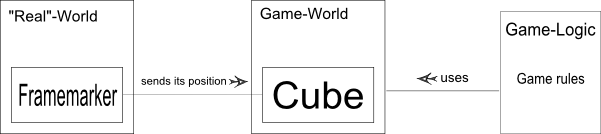
\includegraphics[width=\textwidth]{includes/complexCubeMarkerModel.png}    
        \caption[Separated Cube-Marker model]{Simple visualization of the separated model.} 
        \label{fig:complex_cube_marker_model} 
\end{figure}

In this model the markers would pass their transforms to the cubes as function parameters. The cubes would then use these to position them selfs in the game world. This model was not the one we went with but it had many options we had to consider:
\begin{itemize}
  \item We could use a different marker to show where the table is and use this to position and rotate the cubes. The cubes can not be lower than the table and they have to lay flat if they are on the table. Considering the instability of frame-markers (we couldn't just use one) and the difficulty of getting the markers recognized (we couldn't use many), frame-marker were pretty much out of the picture. We could use an image-target as a tablecloth. We tried to set up image-targets, but we couldn't get the targets recognized. It could have been a problem with the paper or size, scale, resolution of the image, lighting conditions, setup and so on, but we decided to drop this.
  \item We could have used more than one marker for each cube, put one on each side and average their transforms. This could have helped make the cubes just a little more visible and stable, but it would create a lot of complexity. Using several markers increases the chance of one of them, particularly the ones that are the least visible to mess up the cubes position even if it's not as much due to the averaging. The complexity would be a lot extra work for us to create handling for all those optional markers and for the devices that have to run the program. Since we were developing for tablets and cellphones we tried not to push the limits to much. It wouldn't help all that much since the cubes are massive objects, and really just need one clearly visible marker to be placed perfectly in the game world.
  \item We could handle the activation and deactivation of the cubes our selfs. This we did actually attempt to do. The result was a lot more stable, pretty and even colorful than the standard Vuforia- / Unityway, but much worse in relation to game-play. The cubes would freeze in place on the screen, for short periods of time making it hard to see what was going on behind them and generally just feel very unnatural to play with. We could have done the same as Vuforia to hide them when the markers aren't visible, but then there wouldn't really be a point in doing it and we didn't manage to make manual version as natural. 
  \item We could show transparent cubes where the markers were, manipulate the transforms and then place the cubes there with no transparency. But this would just be an excuse, a way to make up for the unnatural way of handling the input and it would probably just distract the player from the game it self.
\end{itemize}


\subsection{Solution}
In the end we decided to use the standard way, with a way to easier set different parents than the frame-markers and use filtering on the game-world state before testing for goal completion, rather than modifying the cubes positions before displaying them to the user. We found this gave the cubes fairly natural and more relate-able and forgivable behavior and to be better for playing the game as players. This way shows the player the instable recognition of the markers, allowing him to adapt to it while keeping the world state that is being tested with the game rules to be a little more stable than it seems. Not by using individual manipulation, but by universal filtering to make the state stable.

	\chapter{Development changes and decisions}
		\label{chap:Developmentchangesanddecisions}
		Following is a list of decisions and changes we as a group made during the development of this project in chronological order.

\begin{enumerate}
	\item 09.jan: As many as possible mini games should be created in a dynamic way.
	\item 09.jan: Graphics for the system does not have to be more advanced than what is shown in the design document.
	\item 09.jan: The cubes need only to have basic collision between others to achieve the functionality we need for the games.
	\item 09.jan: Our focus should be on making as many games as possible within the framework and not on making  a few perfect ones.
	\item 24.jan: We decided to shift our focus to be more on the framework itself and not the games within the framework.
	\item 30.jan: Costas wants us to implement a variation of the mobile app Wooords to replace a few of the other mini games.
	\item 31.jan: We decide to look into the implementation of Wooords at a later date in the development as it is a interesting game and will enhance the finished app since it is not similar to the other mini games.
	\item 10.feb: The group, along with Costas have decided to drop the memory mini game and the path mini game described in the design document.
	\item 17.feb: In the design document it implies that the loading screens should have all time leader board and a high score for the player. This is not consistent with the rest of the design document nor with our planning document and it was decided to instead have a high score for the current player on the loading screen instead.
	\item 06.mar: The design of the boxes is set in the inspector during the making of the game in Unity, the design can therefore not be changed during runtime.
	\item 10.mar: We decided to look into detached / integrated use of a AR library.
	\item 18.mar: Pictures that will be used as textures on the cubes must be in a folder called "/Resources/BoxDesign/" to be able to properly load them since we are not able to extract the path of where a texture is stored on disc.
	\item 27.mar: The levels for mini games will be procedural generated unless you want to make a Wooords mini game, where the levels will be read from file since these levels can not be easily randomly generated.
	\item 29.apr: The restart button have been removed from the pause screen.
\end{enumerate}

\subsection{Framework instead of games}
In the beginning we wanted to make sure that we would be able to create all the games described in the design document, and after looking into how we should structure the programs and what scripts and the like could be shared between each of the mini games we realized that on the programming side of them there was little difference. We therefore decided upon focusing making a framework to work within instead of making each mini game special.

\subsection{Implementing a word game instead}
Shortly after beginning development and starting testing of the \gls{Frame Marker} we realized that the mini game \#5: Memory cubes as it was described in the design document was not implementable. Playing the game would make the player turn the cube upside down in the best case scenario or covering the frame marker and then turn the cube in the worst case. This caused us a lot of problems because of the way that Vuforia controls its frame markers. What Vuforia does when it is not tracking a frame marker or it loses the tracking is to deactivate the frame marker in the scene hierarchy which makes us unable to access any information contained within both the frame marker object itself and its children. This meant that we had no reliable way to detect if the player turned a cube to see the hidden mark under the cube or if it was simply re-detected by the tracker due either by the player obscuring the marker or something else obscuring the marker or the marker just being lost for a few frames. We brought this issue to our employer and after a short discussion we came to the conclusion to implement our own version of the mobile game Wooords and not make the mini game \#5: Memory cubes and also to not make mini game \#6: Path as the game was deemed % nu nu nu
Woords is a game where the player is presented with a jumble of words and a theme. The goal is to find as many or all the words in the level by combining the letters to make words.


\subsection{Dropping leader-board}
In the original design document we got there was mention of having the loading screen both instructions for the game and a global leader-board. Unity does not work well with net based activities 

\subsection{Putting textures in a special folder}
This decision is due to a limitation in Unity. When you place a object in the object field in the inspector it will give us a new instance of that object, in this case a texture. What it does not give us is where it is stored. This would not be a problem if Unity was able to serialize our data, but since we are storing our objects as a JSON object due to Unity not being able to serialize it we have to store it ourself and the name of the texture is the only data we can rely on. The name however does not include the path of where the object is stored, so when we are extracting the data back from JSON objects into textures we only have the name of the texture. So to avoid any confusion of duplicate names and avoiding searching for the texture we constrict the location of where it can be placed into a sub-folder in the Resources folder of Unity.

\subsection{Procedural generation over predetermined levels}
In the beginning of the development we were uncertain about whether we should create levels for the mini games with code or if it should be crafted by hand. We initially went for the possibility of both, however after discussing it with our employer we came to the conclusion that as many of the games as possible should have generated levels. The only mini game that is not suitable for random generation is mini game \#7: Wooord game, the Wooord game has a single file for each set up starting with the overall theme (example is: animal, this means that all the words are animal related), followed by a comma separated sequence of what words should be on the cubes and on the line under is a comma separated list of words that can be created with those words. To create more levels the file just have to continue with a new sequence of letters for the cubes to have and a new line of words that can be created.

\subsection{The restart button has been removed from the pause screen}
\todo{Jakob kan skrive om hvorfor den f\o{}rst \o dela alt, men at vi senere fikset den.}


\part{Product}

	\chapter{Visual}
		\label{chap:visual}
		% Visual

\begin{figure}[h]
	\centering
	\begin{minipage}{.5\textwidth}
		\capstart
		\centering
		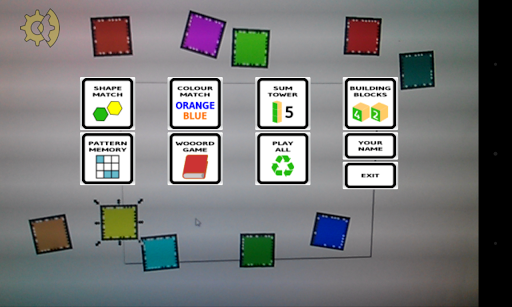
\includegraphics[width=0.9\textwidth]{images/main_menu.png}
		\vspace{-10pt}
		\caption{Screenshot of the main menu.}
		\label{fig:main_menu}
	\end{minipage}%
	\begin{minipage}{.5\textwidth}
		\capstart
		\centering
		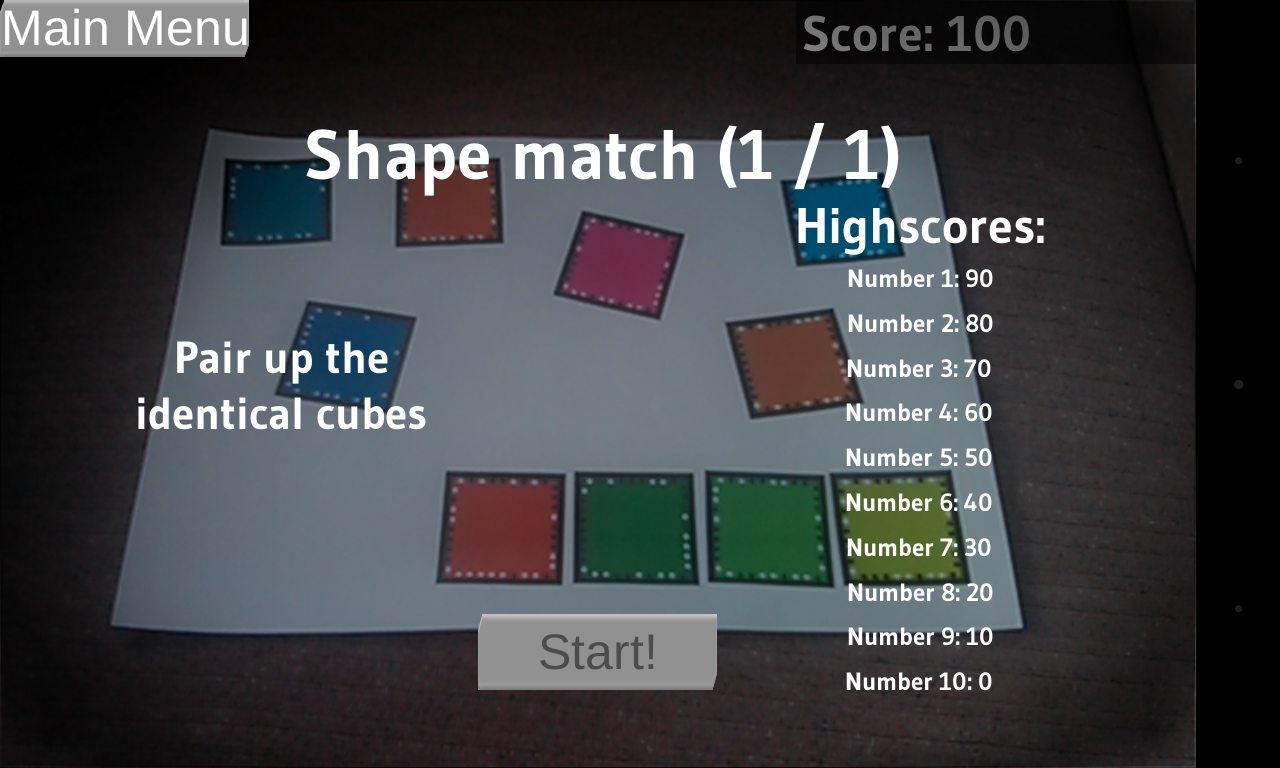
\includegraphics[width=0.9\textwidth]{images/loading_screen.png}
		\vspace{-10pt}
		\caption[Screenshot of a loading screen.]{Loadingscreen for a game.}
		\label{fig:loading_screen}
	\end{minipage}%
\end{figure}

\paragraph{}
The main menu consists of buttons that leads to each minigame with each button having both the name of the corresponding
minigame and a small illustration that gives the user a hint to what the user will do.
There is also the "YOUR NAME" and "EXIT" buttons. The "YOUR NAME" button will take the user to a new screen with a input field 
for changing or setting their username. The "EXIT" button will exit the application.
The camera is always running and we can see the input being rendered to the background.

\paragraph{}
The second picture, \autoref{fig:loading_screen}, shows one of our loading screens, in this case it is the loading screen for \nameref{game:shape_match}.
The loading screens are comprised of two main elements and three smaller elements.
The main elements are the highscore list to the right and a description on the left.
These will introduce the user to what the goal for the minigame is and hopefully encourage the user to do their best every time to improve the highscore.

The smaller elements are as follows. A titlebar showing game title, current level and how many levels there are in total in that game.
A button in the top left corner that lets the user return to the main menu. Lastly there's the "Start!" button that begins the game.

\begin{figure}[h]
	\centering
	\begin{minipage}{0.48\textwidth}
		\capstart
		\centering
		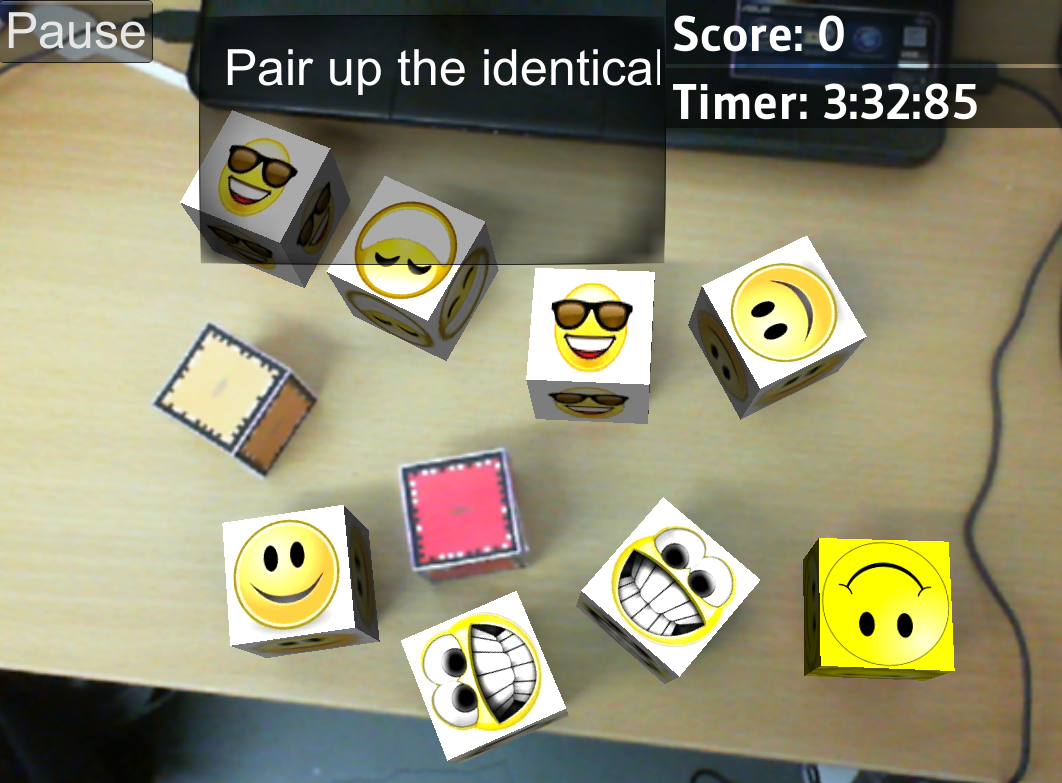
\includegraphics[height=110pt]{images/match_cubes_old}
		\caption[Previous UI in game.]{Early user interface.}
		\label{fig:early_user_interface}
	\end{minipage}
	\begin{minipage}{0.48\textwidth}
		\capstart
		\centering
		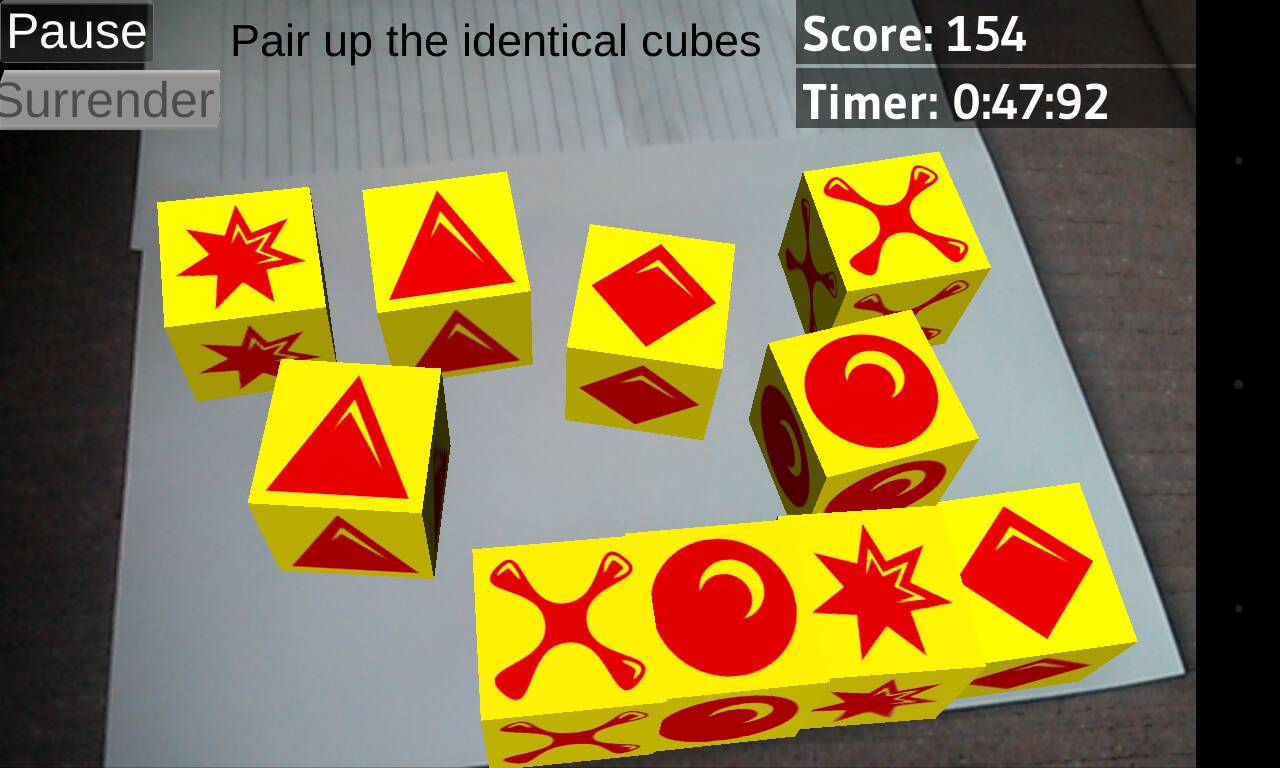
\includegraphics[height=110pt]{images/match_cubes_new}
		\caption[Current UI in game.]{Current user interface.}
		\label{fig:current_user_interface}
	\end{minipage}
\end{figure}

\paragraph{}
\autoref{fig:early_user_interface} and \autoref{fig:current_user_interface} shows our current UI and what we had in the beginning.
Our first version used the default Unity style for both buttons and info boxes.
While it is functional it is not very nice to look at and is too distracting in a environment such as this.
To rectify this we created our own UI styles to use instead of the default.
By removing as many distracting elements from the UI as possible we leave much more space open so the user can use more of the
screen to look for the cubes without having the UI getting in the way.



\section{Program flow chart}

\begin{figure}[h]
	\capstart
	\centering
	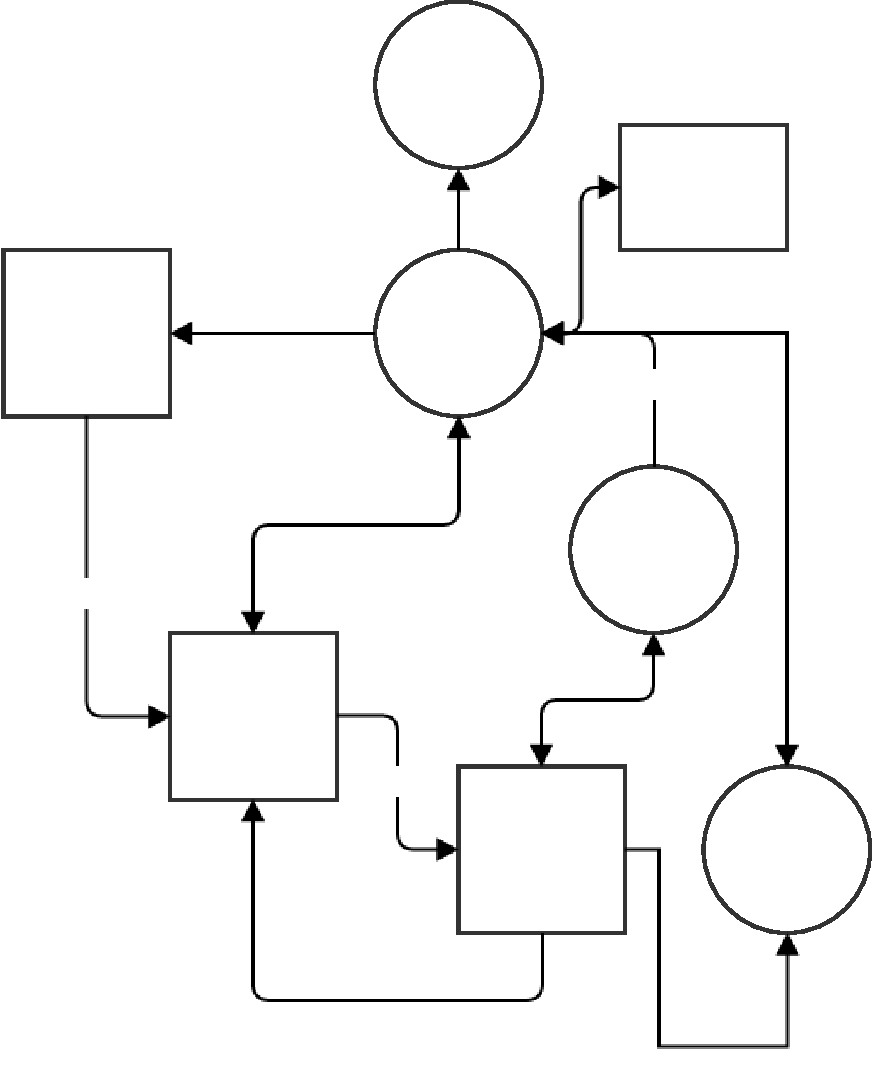
\includegraphics[width=0.8\textwidth]{images/user_flow_chart}
	\caption[Program flow chart]{How a user maneuvers in the program.}
	\label{fig:program_flow_chart}
\end{figure}

Upon starting the program the user is presented with the main menu.
The main menu consists of four different types of buttons.

The first buttons are those that lead to a single mini-game.
When clicked, the player will be taken to the loading screen of the appropriate mini-game. There, the player can read instructions for the game and see current high-scores for that game.
After clicking the play button, the user can start to play the game and the time that effect score will run. While playing, the user can always press pause to get a break.
If the user presses the pause button a pause screen is shown with the options of resuming the game, restarting from level one or go back to the main menu.

When completing a level, the user is taken back to the loading screen if there are more levels left. Otherwise score and position in the high-score list are shown.
From that point the user can only go back to the main menu.

The second type of button are one that is named "Play all games". When the user presses this button it will play all the available mini-games in sequential order.

The next button type are one that changes user. It is called "Change username". When pressing this the user will be presented with a input field where a name can be entered.
This will change the username that is shown in the high-score list. The same name are also used in the logging that are sent to a server.

The last button type will end the program. We only need one of this and it is simply called "Quit".

	\chapter{Application data}
		\label{chap:application_data}
		\todo{Which data are stored in the app and which data is sent to the
		network? This should be a summary of what we have written under
		development.}

\subsection{Data kept locally}
\subsection{Data sent to server}

	\chapter{Feedback}
		\label{chap:feedback}
		\begin{itemize}
	\item A friend from F\o{}rde tried the app on his Samsung S5. This caused his phone to restart. When he tried the app after it's restart, the phone only replied that the program had stopped.
	\item There has been reported that it was hard to install the program from
	our webpage. To do so, one need to accept programs from "unsafe" sources
	that are not on Google Play.
	\item People have asked for the app both for iOS and Windows Phone. We have
	tried to port cogARC to these platforms, but never succeeded. There may be
	some APIs and features that are not availible in the Unity free edition.
	For Windows Phone the webcam is not availible
	\cite{GettingStartedWindowsPhoneBuildUnity}, so that may be one of the
	problematic factors.
	\item Someone was observed to connect the frame markers by dragging
	on the screen from one of them to the other. This is probably since it is a
	new technology and may be most prominent the first time a person tries it.
	\item By trying on a smart phone someone was observed to hold it quite high
	in a sitting position. The reason was to see all the frame markers at the 
	same time. It was an uncomfortable position and the player started to 
	recognize it in their back. This was played without cubes, but with flat
	markers on the table. It may not be a problem when playing it as the
	employer have described -- with cubes in a sitting position with a tablet
	in front(bigger screen).
	\vspace{8pt}
	\item \nameref{game:pattern_memory}:
		\vspace{-8pt}
		\begin{itemize}
			\item Friend did not see the pattern in the corner when it
			started. A possible solution could be to put it at the middle of
			the screen to make it easier to see.
			\item Someone experienced that the game said the solution was both
			right and wrong at the same time. Algorithm optimization needed.
		\end{itemize}
	\item \hyperref[fig:pair_games]{Pair games}: Some got paired up without the user recognizing it. This
	we have seen before. A possible solution could be to show how many
	pairs that are left. On \nameref{game:shape_match}, it could e.g be 
	pictures of those that are left.
	\item \hyperref[subsec:vuforia]{Vuforia}: Marker recognition not good
	enough. Problem with seeing	markers are often problematic.
	\item General: Player felt frustrated and confused when not understanding
	the games. This changed upon completion of a level, where instead there 
	were rewarding feelings of joy and victory (\nameref{game:pattern_memory}).
\end{itemize}

	\chapter{Future Development}
		\label{chap:future_development}
		There are many ways to work further with the software we have started on.
The first thing we will propose is to do proper testing and fix the bugs that
will show up. Testing should uncover whether the functionality works as 
intended or not. It should also try to see if the games work as intended.

Onother area that needs to be improved are the graphical user interface (GUI).
It will be a great id\'ea to get professional interaction designers to specify
and create the user interface. The current GUI are responsive to some extent, 
but it have proved not to be good enough. This is highly encouraged to get 
done.

\paragraph{}

When it comes to advancing the software, there are some points we would like 
to mention. One exciting thing to try is to port cogARC to wearable glasses.
Since the original plan was to implement the program for the \gls{Meta 
SpaceGlasses}, these will probably be good to try it on. From their webpage
\cite{MetaSpaceGlasses}, they now, at the 13th of May 2014, claims that new 
orders will start shipping in September. We will expect Kickstarter supporters 
to receive the product a bit before that, so it might be ready to test in only
a few months time if anyone would implement it.

Another advancement is to do something with the tracking and flickering of the 
markers. This is a disturbing factor in the games and would enhance the game
experience if it were fixed. One way is to use an other tracking library than
Vuforia, but there may be tricks that can be done locally to reduce the 
problem. One way can be to handle the input from the library in a more advanced
way.

\paragraph{}

From a more academic perspective, it would be good to look more into the actual
research value of cogARC. When looking at it from that angle, there may show up
several ways to enhance the software. Logging may change in what data that are
being logged and how the data is filtered, stored and used.

New games may be added to investigate in other cognitive functionalities than 
those that are already there. Some of the games that are implemented may be
filtered out, while others may change if they does not serve their purpose well.



\part{Summary}

	\chapter{Conclution}
		\label{chap:conclution}
		\subsection{What we set out to do}

\begin{description}
	\item \todo{Comment on them. They are only copied from the planning document...}

	\item[Result goals]\ 
	\begin{itemize}
		\item 7 games.
		\item Adaptable framework.
		\item Viable bachelor thesis.
		\item Combine physical cubes and digital structures.
	\end{itemize}
	From the initial plans some game-ideas were dropped for technical issues and some were dropped because they were found necessary and uninteresting and some were added to take their place. 
	This selection-process was done over time early in the project and we completed all the games we decided to do. 
	We also made code for one of the games we dropped, but this game was not put into the application and was never properly tested. 
	We can create a new simple game type in 1-2 days.\\
	The framework we made is flexible beyond what was required to make the requested games. 
	The rules of games can easily be changed in Unity. 
	There are several options for changing the difficulty of games, such as setting time limits, setting number of cubes used to form solutions and setting number of levels. 
	For the word-game \ref{game:wo0ord_game} the file containing the tasks can easily be changed. 
	The game description can be changed and the score system can to some degree be tweaked in the inspector. 
	The main-menu is not as flexible and it is the most problematic area when wanting to expand the application to have more than the 6 base games or more series than the all game series. 
	In the scripts it's fairly easy to create long series of games. It takes a little more work to create buttons in the main-menu for starting them.\\
	\todo{did we do enough work?}
	yes we believe we did.\\
	We turned the volatile environment seen by the cameras of the real world into fairly stable arrays and lists and tested them against preset and randomly created states. 
	Some buggy behavior occurs, but most of this is because the images from the camera are too bad for the trackers or because of Vuforias tracking algorithms.\\

	\item[Effect goals]\ 
	\begin{itemize}
		\item Supporting research.
		\item Experience with a game engine.
		\item Experience with a longer development process.
		\item Experience with digital space linked to reality
	\end{itemize}
	We cannot really say at this point how well our product will support the research, but our employer stated that he was pleased with the product and we were able to meet most of the requirements for logging events. 
	So we reckon it will be at least a little useful.\\
	We haven't had a lot experience with large projects and they have all been in different environments, coding languages and with different tools. 
	So we had a lot of trouble in the beginning of the project with structure, setting up the scene hierarchy, where to put scripts and making scripts communicate. 
	As we implemented new features we went over the structure several times, improving it a little each time. 
	The Unity project still shows signs of structural weaknesses we chose not to remove because it would mean a lot of refracturing-work. 
	We believe that in future projects in Unity and similar we will be able to set much better structure because of the experience we gained in this project.\\
	We didn't really explore the AR field as much as our supervisor wanted us to, but we studied the possibilities. 
	If the technology had been better we might have gone much deeper in this direction.


\end{description}


\subsection{What we did}

\subsection{How we did it}
\todo{Evaluate the groupwork.}

\subsection{Reflection}
	\todo{End status report: What works, what was dropped, what could need more time.}
Everything works.
Testing need more time.

	\chapter{Afterword}
		\label{chap:afterword}
		\input{includes/cogARC_afterword}


\todo{Remove this when people know how to use glossaries or before delivery}
Here is an example on how to use glossaries. We can for example use the word
\gls{ECMAScript}. Now we get the text ECMAScript with a link to the glossary
list. In the glossary list there will also be a link to where this is 
referenced in the document. The same applies for \gls{serialization}.

Example of references inside the document:
	Here is a reference to chapter \ref{chap:related_work}.
	Here is a reference with the name of the chapter \nameref{chap:related_work}



\part{Appendices}

\appendix %after this line all chapters will have leters instead of numbers
%\appendixpage
%\addappheadtotoc

% References
\bibliographystyle{classes/gucthesis}
\bibliography{includes/cogARC_bibliography}

% Glossary list
\printnoidxglossary[sort=word]

\chapter{Time management}
	\label{appx:time_management}
	\todo{Put the data from Toggl here}





% Examples
% \chapter{Packages}
\label{chap:packages}

The \texttt{gucthesis} is built upon the standard \LaTeX\
\texttt{report} class. All commands from the \texttt{report} class can
be used, with the two exceptions of \verb+\subsubsection+ and
\verb+\paragraph+. This is because there should only be three
levels of headings according to the guidelines~\cite{GUCMaster}.

\section{Packages Used by gucthesis}
\label{sec:packages}

In addition to the \texttt{report} document class,
\texttt{gucthesis} makes direct use of the following packages
that must hence be present:
\begin{description}
	\item[geometry:] used for setting the sizes of the margins and
  	headers.
	\item[fontenc:] used with option \texttt{T1} for forcing the Cork font
  	encoding (necessary for the Charter font).
	\item[charter:] load Charter as the default font.
	\item[euler:] load the Euler math fonts.
	\item[babel:] to load language specific strings. Reasonable options
	  include \texttt{british}, \texttt{american}, \texttt{norsk},
	  \texttt{nynorsk} and \texttt{samin}.
\end{description}

\section{Other Relevant Packages}
\label{sec:otherpackages}

The author of a thesis might want to use a bunch of different packages
to those described in Section~\ref{sec:packages} in order to have all features needed for their document. 
In particular, it is advised to use the following:
\begin{description}
	\item[inputenc:] to allow \LaTeX\ to use more than 7-bit ASCII for its
	  input. Most often, the option \texttt{latin1} will do.
	\item[graphicx:] to include graphics.
	\item[hyperref:] this is a very nice package that makes cross links in
	  pdf documents. Use with option \texttt{dvips} or \texttt{pdftex}
	  in accordance with the driver that you use. Unfortunately, hyperref
	  is not completely bugfree\dots
\end{description}

% \chapter{Structural Elements}
\label{chap:structural}

The title of the thesis should be set using the \verb+\thesistitle+
command, and the date of the thesis should be set using the
\verb+\thesisdate+ command. This makes the title and date appear in
the running header, like in this document.

\section{Page Layout}

The geometry of the page has been set using the \verb+\geometry+
command.

\section{Fonts}

Due to limited \LaTeX\ support for the Georgia font, Charter has been
chosen instead. For mathematical formula, the Euler fonts are used,
since they blend more nicely with the Charter than the standard
\LaTeX\ fonts: 
$$
 f(x) = \int_0^x g(\tau)\,d\tau
$$

For inline math you can use $\backslash{}($ and $\backslash{})$ for example \( f(x)= \frac{x^2}{1+x^2} \).  
This also allows you to use $\slash$ and $\backslash$. You need to include the \{\} when you want the special
character to have other letters immediately after it.

\section{Sectioning Commands}

The standard \LaTeX\ sectioning commands are used for both numbered
and unnumbered sections. The top level is given by the \verb+\chapter+
command. This starts a new right page. The two lower levels are
obtained using the \verb+\section+ and \verb+\subsection+ commands.
The standard \LaTeX\ \verb+\subsubsection+ and \verb+\paragraph+
commands have been disabled since their use is not encouraged by the
thesis guidelines. When you use these they will not be given numbers.  
They still appear in the document with highlighting but not in the 
table of contents.

\subsection{The subsection}

This is an example of a subsection.

\subsubsection{The subsubsection}

This is an example of a subsubsection.

\paragraph{The paragraph}

This is an example of a paragraph with a heading.

\section{Floats (Figures and Tables)}
\label{sec:floats}

Figures are placed in the \texttt{figure} environment. An example is
shown in Figure~\ref{fig:example}. %notice the ~ in between figure and the \ref. it stops latex from splitting the number and word over a line.
Tables are placed in the \texttt{table} environment. An example is given in
Table~\ref{tab:example}. Figures and tables float freely around in the
document in accordance with standard \LaTeX\ behavior.

\begin{figure}[tbp]  %t top, b bottom, p page | you can also use h to try to get the figure to appear at the current location
  \centering
  
\includegraphics[width=.5\textwidth]{example_fig}
  \caption[An example figure.]{An example figure. If the caption is
    shorter than one line, it is centered. If it goes over more than
    one line, it is left and right justified. Furthermore, it is
    suggested that an alternative short caption is given in order to
    produce a good list of figures.}
  \label{fig:example}
\end{figure}

\begin{table}[tbp]
  \centering
  \begin{tabular}{c|c}
    Age  & IQ  \\ 
    \hline
    10   & 100 \\
    20   & 100 \\
    30   & 150 \\
    40   & 100 \\
    50   & 100
  \end{tabular}
  \caption{An example table.}
  \label{tab:example}
\end{table}

The captions are placed \emph{below} both for the figures and the
tables. The caption is set in 9pt. If the caption is shorter than one
line, it is centered.

\section{Quotes}
\label{sec:Quotes} % this allows you to refer to this section number using \ref{sec:Quotes}

Quotes are inserted using the standard \LaTeX\ \texttt{quote}
environment. The environment has been changed so that a 9pt font is
used:

\begin{quote}
  ``And I looked, and, behold, a whirlwind came out of the north, a
  great cloud, and a fire infolding itself, and a brightness was about
  it, and out of the midst thereof as the colour of amber, out of the
  midst of the fire. Also out of the midst thereof came the likeness
  of four living creatures.''
\end{quote}

\section{Lists}
\label{sec:lists}

Point lists and enumerated lists are made by using the standard
\texttt{itemize} and \texttt{enumerate} environments, respectively.
The spacing is going to be changed in accordance with the specification. For
\texttt{itemize}, the results look like this:
\begin{itemize}
	\item First item.
	\item Second item. Here I will put some long text, just to illustrate.
	  Here I will put some long text, just to illustrate. Here I will put
	  some long text, just to illustrate. Here I will put some long text,
	  just to illustrate.
	\item Third item also has subitems:
	  \begin{itemize}
		  \item First subitem.
		  \item Second subitem.
		  \item Third subitem.
	  \end{itemize}
\end{itemize}
and for \texttt{enumerate} like this:
\begin{enumerate}
	\item First item.
	\item Second item. Here I will put some long text, just to illustrate.
	  Here I will put some long text, just to illustrate. Here I will put
	  some long text, just to illustrate. Here I will put some long text,
	  just to illustrate.
	\item Third item also has subitems:
	  \begin{enumerate}
		  \item First subitem.
		  \item Second subitem.
		  \item Third subitem.
	  \end{enumerate}
\end{enumerate}

You may also want to use descriptive lists
\begin{description}
	\item[First] the first item.
	\item[Second] the second item. Here I will put some long text, just to illustrate.
	  Here I will put some long text, just to illustrate. Here I will put
	  some long text, just to illustrate. Here I will put some long text,
	  just to illustrate.
	\item [What now] the third item also has subitems:
	  \begin{enumerate}
		  \item First subitem.
		  \item Second subitem.
		  \item Third subitem.
	  \end{enumerate}
\end{description}


\section{Bibliographic References}

You should cite articles~\cite{Askvall1985}, books~\cite{Card1983},
anthologies~\cite{Lancaster1985} and web publications~\cite{Meldon1997}
like this. There is always an issue referencing web pages. Currently
we suggest that you use the HiG Website~\cite{HiG:Website}.


A particular bibliography style file for GUC named
\texttt{gucthesis.bst} has been developed based upon the
standard Bib\TeX\ \texttt{unsrt} style.


% \chapter{Meetings}

You can include an Appendix of the log of your meeting for example

% \GUC, 
% \comment{so what}

% \todo{task \#1}
% This is a todo-task we need to get done.


\end{document}